\documentclass[english,t]{beamer}
%\documentclass[handout,english]{beamer}

\mode<presentation>
{
  \usetheme{Copenhagen}
  % oder ...
  
%  \setbeamercovered{transparent}
  % oder auch nicht
}

%\usepackage[pdftex]{graphicx}
\graphicspath{{/home/ave/doc/images/}{}{../teranaloppu/}{../metodi/}{../slides/Hartikainen/}{../gphealth/}{../2008_09_RSS2008/}{../gphealth/}{../jyvaskyla2009/}{../nbbc2009/}{../gphealth/hippics/}{../euroheis2010/}{../pubgensens2011/}{../reykjavik2013/}{../liverpool2013/}{../../gpstuff/doc/}{./images/}{../aalto_stochastic/}{figs/}{../Stancon2018Helsinki/figs/}{../../paper/cvapprox/}{../gppa2017/}{../valencia2017/}{../../paper/combine_predictive_distribution/tex/}{../venice2018/figs/}{./figs/}}
\usepackage[T1]{fontenc}
\usepackage[utf8]{inputenc}
\usepackage{times}
\usepackage{amsmath,amsfonts,amssymb}
%\usepackage{euscript}
\usepackage{afterpage}
%\usepackage{picinpar}
%\usepackage{array,longtable}
\usepackage{url}
\urlstyle{same}
%\usepackage{eufrak}
\usepackage{amsbsy}
\usepackage{eucal}
\usepackage{rotating}
\usepackage{bm}
\usepackage{pdfpages}
\usepackage{algorithm}
\usepackage[noend]{algpseudocode}
\usepackage{booktabs}
\usepackage{listings}
\usepackage{lstbayes}
\usepackage{microtype}

\usepackage{natbib}
\bibliographystyle{apalike}

\hypersetup{%
  bookmarksopen=true,
  bookmarksnumbered=true,
  pdftitle={Stan},
  pdfsubject={Bayesian data analysis},
  pdfauthor={Aki Vehtari},
  pdfkeywords={},
  pdfstartview={FitH -32768},
  colorlinks=true,
  linkcolor=navyblue,
  citecolor=navyblue,
  filecolor=navyblue,
  urlcolor=navyblue
}

%%%%%%%%%%%%%%%%%%% for tikz figures %%%%%%%%%%%%%%%%%%%%%%%%%%
\usepackage{ifthen}
\usepackage{tikz,pgfplots}
\usetikzlibrary{matrix}
\usetikzlibrary{calc}
\newlength{\figurewidth}
\newlength{\figureheight}


\def\figpdfdir{./fig/} % directory for pdf-figures
\def\figtikzdir{./tikz/} % directory for tikz-figures 

% this is replacement for the \input command used in the figure-environment which
% takes into account whether pdf is forced
\newcommand{\minput}[2][]{
\ifthenelse{\equal{#1}{pdf}}
	{ \includegraphics{\figpdfdir #2} }
	{ \tikzset{external/remake next} \tikzsetnextfilename{#2} \input{\figtikzdir #2} }
}

% for externalization
\usetikzlibrary{external}
\tikzexternalize[prefix=\figpdfdir] 
\tikzset{external/system call={lualatex
	\tikzexternalcheckshellescape -halt-on-error -interaction=batchmode
	-jobname "\image" "\texsource"}}
    
%%%%%%%%%%%%%%%%%%% for hiding figures %%%%%%%%%%%%%%%%%%%%%%%%%%
\usepackage{color}
\newcommand{\hide}[5][white]{
	% usage: \hhide[color]{vspace,hspace,height,width}
	% note: all measures are relative units measured in \textwidth
	%\begin{minipage}{0.99\textwidth}
	\vspace{#2\textwidth}
	\hspace{#3\textwidth}
	\textcolor{#1}{  \rule{#5\textwidth}{#4\textwidth}  }
	% \end{minipage}
      }

\DeclareMathOperator{\Kfu}{\mathbf{K}_{f,u}}
\DeclareMathOperator{\Kuf}{\mathbf{K}_{u,f}}
\DeclareMathOperator{\Kff}{\mathbf{K}_{f,f}}
\DeclareMathOperator{\iKff}{\mathbf{K}_{f,f}^{-1}}
\DeclareMathOperator{\Kfa}{\mathbf{K}_{f,\tilde{f}}}
\DeclareMathOperator{\Kaf}{\mathbf{K}_{\tilde{f},f}}
\DeclareMathOperator{\Kaa}{\mathbf{K}_{\tilde{f},\tilde{f}}}
\DeclareMathOperator{\Kuu}{\mathbf{K}_{u,u}}
\DeclareMathOperator{\iKuu}{\mathbf{K}_{u,u}^{-1}}
\DeclareMathOperator{\Kau}{\mathbf{K}_{\tilde{f},u}}
\DeclareMathOperator{\Kua}{\mathbf{K}_{u,\tilde{f}}}
\DeclareMathOperator{\Qff}{\mathbf{Q}_{f,f}}
\DeclareMathOperator{\Qaa}{\mathbf{Q}_{\tilde{f},\tilde{f}}}
\DeclareMathOperator{\Qfa}{\mathbf{Q}_{f,\tilde{f}}}
\DeclareMathOperator{\Qaf}{\mathbf{Q}_{\tilde{f},f}}
\DeclareMathOperator{\x}{\mathbf{x}}
\DeclareMathOperator{\f}{\mathbf{f}}
\DeclareMathOperator{\y}{\mathbf{y}}
\DeclareMathOperator{\h}{\mathbf{h}}
\DeclareMathOperator{\uu}{\mathbf{u}}
\DeclareMathOperator{\LL}{\mathbf{\Lambda}}
\DeclareMathOperator{\bb}{\mathbf{b}}
\DeclareMathOperator{\E}{\mathrm{E}}
\def\WAIC{\mathrm{WAIC}}

\newcommand{\kin}{k^{\rm in}}
\newcommand{\kout}{k^{\rm out}}
\newcommand{\gi}{{R_0}}
\newcommand{\eff}{{E_{\rm max}}}
\newcommand{\HN}{{\rm N^+}}
\newcommand{\lN}{{\rm LN}}
\newcommand{\Rss}{R^{\rm ss}}
\newcommand{\invlogit}{\mbox{logit}^{-1}}

% \DeclareMathOperator{\Poisson}{Poisson}
\DeclareMathOperator{\Chi}{Chi}
\DeclareMathOperator{\GP}{\mathcal{GP}}
%\DeclareMathOperator{\N}{N}
\DeclareMathOperator{\KL}{KL}

\DeclareMathOperator*{\argmax}{arg\,max}
\DeclareMathOperator*{\argmin}{arg\,min}
\newcommand{\mb}{\mathbf}
\newcommand{\pkg}[1]{{\fontseries{b}\selectfont #1}}
\newcommand{\proglang}{}
\newcommand{\email}[1]{\href{mailto:#1}{\normalfont\texttt{#1}}}
\newcommand{\doi}[1]{\href{http://dx.doi.org/#1}{\normalfont\texttt{doi:#1}}}
\newcommand{\code}[1]{{\normalfont\texttt{#1}}}

% \DeclareMathOperator{\E}{E}
% \DeclareMathOperator{\VAR}{Var}
% \DeclareMathOperator{\COV}{Cov}
% \DeclareMathOperator{\Prob}{P}
% \DeclareMathOperator{\E}{E}
\DeclareMathOperator{\Var}{Var}
\DeclareMathOperator{\var}{var}
\DeclareMathOperator{\cov}{cov}
\DeclareMathOperator{\logistic}{logistic}
\DeclareMathOperator{\softmax}{softmax}
\DeclareMathOperator{\Multinomial}{Multinomial}
\DeclareMathOperator{\Sd}{Sd}
\DeclareMathOperator{\sd}{sd}
\DeclareMathOperator{\Bin}{Bin}
\DeclareMathOperator{\Poisson}{Poisson}
\DeclareMathOperator{\Beta}{Beta}
\DeclareMathOperator{\logit}{logit}
\DeclareMathOperator{\N}{N}
\DeclareMathOperator{\U}{U}
\DeclareMathOperator{\BF}{BF}
%\DeclareMathOperator{\Pr}{Pr}
\def\euro{{\footnotesize \EUR\, }}
\DeclareMathOperator{\rep}{\mathrm{rep}}

\definecolor{set11}{HTML}{E41A1C}
\definecolor{set12}{HTML}{377EB8}
\definecolor{greenish}{rgb}{0.1333,0.8666,0.1333}
\definecolor{forestgreen}{rgb}{0.1333,0.5451,0.1333}
\definecolor{hutblue}{rgb}{0,0.2549,0.6784}
\definecolor{midnightblue}{rgb}{0.0977,0.0977,0.4375}
\definecolor{navyblue}{rgb}{0,0,0.5}
\definecolor{hutsilver}{rgb}{0.4863,0.4784,0.4784}
\definecolor{lightgray}{rgb}{0.95,0.95,0.95}
\definecolor{section}{rgb}{0,0.2549,0.6784}
\definecolor{list1}{rgb}{0,0.2549,0.6784}
\renewcommand{\emph}[1]{\textcolor{navyblue}{#1}}

%\graphicspath{./pics}

\pdfinfo{
  /Title      (Bayesian data analysis ch7)
  /Author     (Aki Vehtari) %
  /Keywords   (Bayesian probability theory, Bayesian inference, Bayesian data analysis)
}

\parindent=0pt
\parskip=8pt
\tolerance=9000
\abovedisplayshortskip=0pt

%\renewcommand{\itemsep}{0pt}
% Lists
\newenvironment{list1}{
   \begin{list}{$\color{list1}\bullet$}{\itemsep=6pt}}{
  \end{list}}
\newenvironment{list1s}{
  \begin{list}{$\includegraphics[width=5pt]{logo.eps}$}{\itemsep=6pt}}{
  \end{list}}
\newenvironment{list2}{
  \begin{list}{-}{\baselineskip=12pt\itemsep=2pt}}{
  \end{list}}
\newenvironment{list3}{
  \begin{list}{$\cdot$}{\baselineskip=15pt}}{
  \end{list}}

\setbeamertemplate{navigation symbols}{}
\setbeamertemplate{headline}[default]{}
\setbeamertemplate{headline}[text line]{\insertsection}
\setbeamertemplate{footline}[frame number]


\title[]{Bayesian data analysis}
\subtitle{}

\author{Aki Vehtari}

\institute[Aalto]{}
 
\date[]{}

%\beamerdefaultoverlayspecification{<+->}

\begin{document}

\begin{frame}
  
   {\Large\color{navyblue} Chapter 7}

   \begin{list1}
   \item 7.1 Measures of predictive accuracy
   \item 7.2 Information criteria and cross-validation
     \begin{list2}
     \item Instead of 7.2, read:\\
       Vehtari, A., Gelman, A., Gabry, J. (2017). Practical Bayesian
       model evaluation using leave-one-out cross-validation and
       WAIC. Statistics and Computing. 27(5):1413–1432.
       \href{http://arxiv.org/abs/1507.04544}{arXiv preprint}.
     \end{list2}
   \item 7.3 Model comparison based on predictive performance
   \item 7.4 Model comparison using Bayes factors
   \item 7.5 Continuous model expansion / sensitivity analysis
   \item 7.5 Example (may be skipped)
   \end{list1}

\end{frame}

\begin{frame}
  
   {\Large\color{navyblue} Model assessment, selection and inference after selection}

   \begin{list1}
   \item Extra material at \url{https://avehtari.github.io/modelselection/}
     \begin{list2}
       \item Videos, Slides, Notebooks, References
       \item The most relevant for the course is the first part of the
         talk ``Model assessment, comparison and selection at Master
         class in Bayesian statistics, CIRM, Marseille''
     \end{list2}
   \end{list1}

\end{frame}
 
\begin{frame}{}

  {\Large\color{navyblue} Predicting concrete quality}

  \begin{center}
    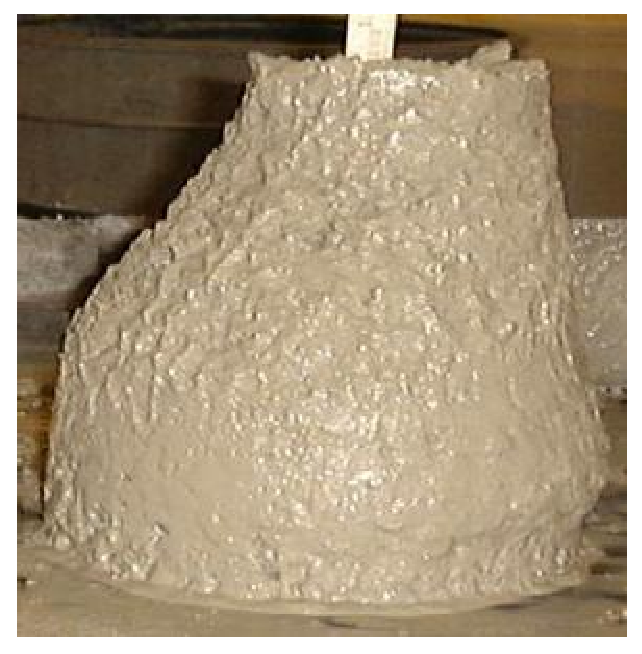
\includegraphics[width=5cm]{slump1b.eps}
  \end{center}
  
\end{frame}

\begin{frame}{}

  {\Large\color{navyblue} Predicting cancer recurrence}

  \begin{center}
    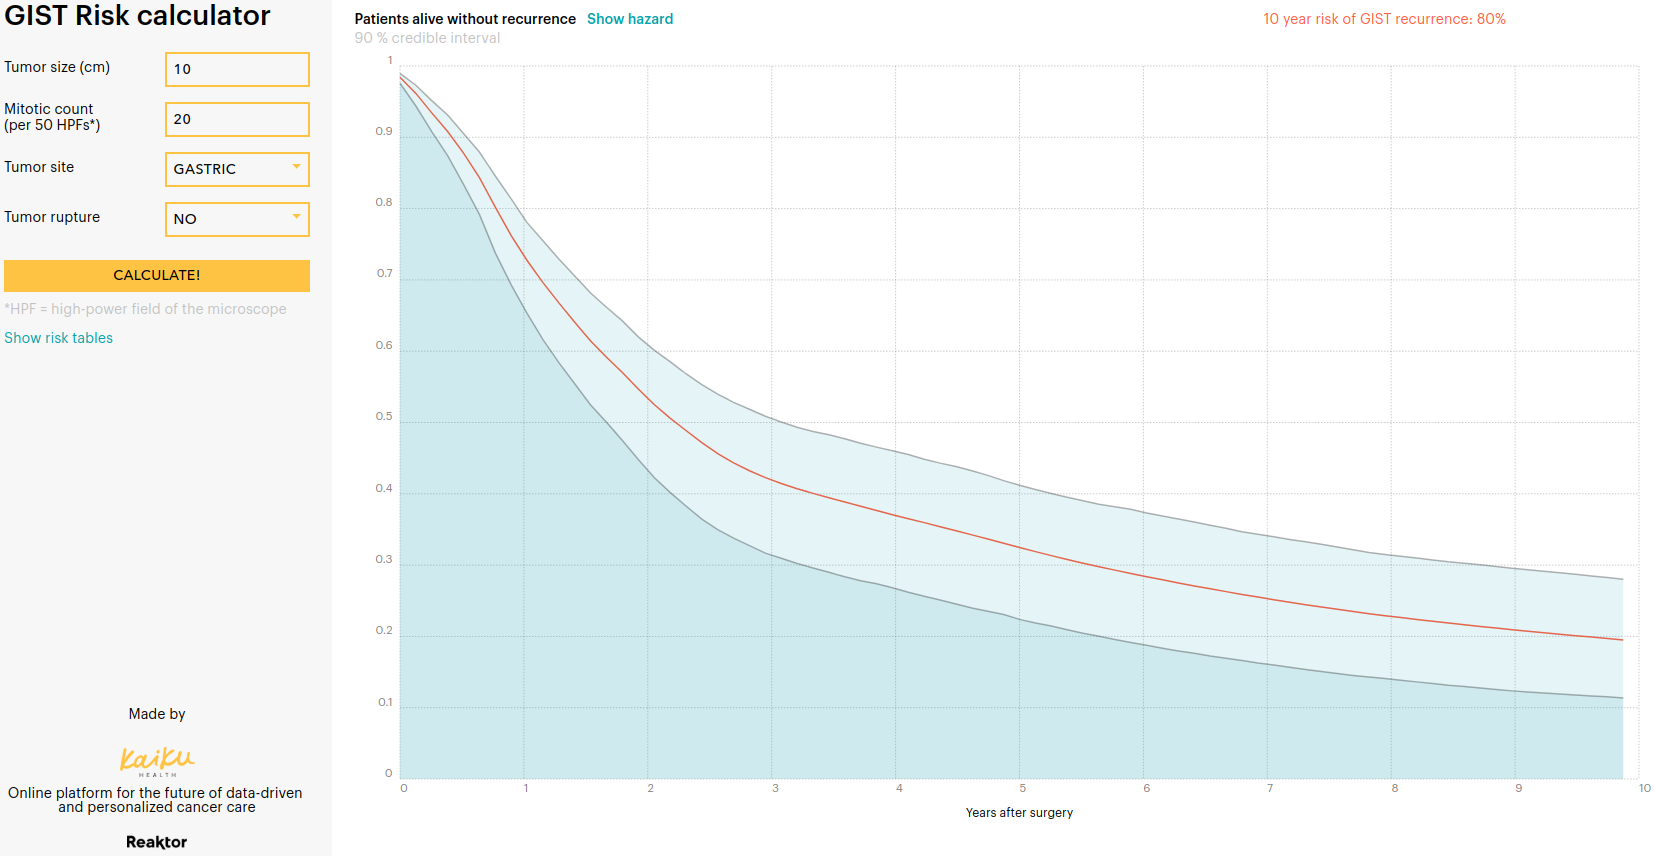
\includegraphics[width=11.5cm]{gistrisk.png}
  \end{center}
  
\end{frame}

\begin{frame}
  
  {\Large\color{navyblue} Predictive performance}

  \begin{itemize}
  \item<1-> True predictive performance is found out by using it to make
    predictions and comparing predictions to true observations
    \begin{itemize}
      \item external validation
    \end{itemize}
  \item<2-> Expected predictive performance
    \begin{itemize}
      \item approximates the external validation
      \end{itemize}
    \end{itemize}

\end{frame}

% \begin{frame}{}

%   {\Large\color{navyblue} Model assessment, comparison, selection and averaging}

%   \begin{list1}
%   \item Modeling complex phenomena with models that
%     are much simpler than the nature ($M$-open)
%   \item<2-> Decision theoretical approch in spirit of
%     \begin{list2}
%     \item Lindley, Box, Rubin, Bernardo \& Smith, etc.
%     \end{list2}
%   \end{list1}
  
% \end{frame}

\begin{frame}
  
  {\Large\color{navyblue} Predictive performance}

  \begin{itemize}
  \item We need to choose the utility/cost function
  \item Application specific utility/cost functions are important
    \begin{itemize}
      \item eg. money, life years, quality adjusted life years, etc.
    \end{itemize}
    \pause
  \item If are interested overall in the goodness of the predictive distribution,
    or we don't know (yet) the application specific utility, then
    good information theoretically justified choice is log-score
      \begin{align*}
        \log p(y^{\text{rep}} | y, M),
      \end{align*}
\end{itemize}

\end{frame}

\begin{frame}{}
  
  {\Large\color{navyblue} Outline}
  
  \begin{list1}
  \item What is cross-validation
    {\color{gray}
  \begin{list2}
    \item Leave-one-out cross-validation (elpd\_loo, p\_loo)
    \item Uncertainty in LOO (SE)
    \end{list2}
    }
  \item When is cross-validation applicable?
    {\color{gray}
    \begin{list2}
    \item data generating mechanisms and prediction tasks
    \item leave-many-out cross-validation
    \end{list2}
    }
  \item Fast cross-validation
    {\color{gray}
    \begin{list2}
    \item PSIS and diagnostics in loo package (Pareto k, n\_eff, Monte Carlo SE)
    \item K-fold cross-validation
    \end{list2}
    }
  \item {\footnotesize Related methods (WAIC, *IC, BF)}
  \item Model comparison and selection (elpd\_diff, se)
  \item Model averaging with Bayesian stacking
  % \item<2-> Part 2: Projective Inference in High-dimensional Problems:
  %   Prediction and Feature Selection
  \end{list1}
   
\end{frame}

\begin{frame}[fragile]

  {\Large\color{navyblue} Stan and {\tt loo} package}

  {\scriptsize
\begin{lstlisting}
 Computed from 4000 by 20 log-likelihood matrix

         Estimate  SE
elpd_loo    -29.5 3.3
p_loo         2.7 1.0
------
Monte Carlo SE of elpd_loo is 0.1.

Pareto k diagnostic values:
                         Count Pct.    Min. n_eff
(-Inf, 0.5]   (good)     18    90.0%   899       
 (0.5, 0.7]   (ok)        2    10.0%   459       
   (0.7, 1]   (bad)       0     0.0%   <NA>      
   (1, Inf)   (very bad)  0     0.0%   <NA>      

All Pareto k estimates are ok (k < 0.7).
See help('pareto-k-diagnostic') for details.

Model comparison: 
(negative 'elpd_diff' favors 1st model, positive favors 2nd) 

elpd_diff        se 
     -0.2       0.1 
\end{lstlisting}
}

\end{frame}


\begin{frame}{}

  \only<1>{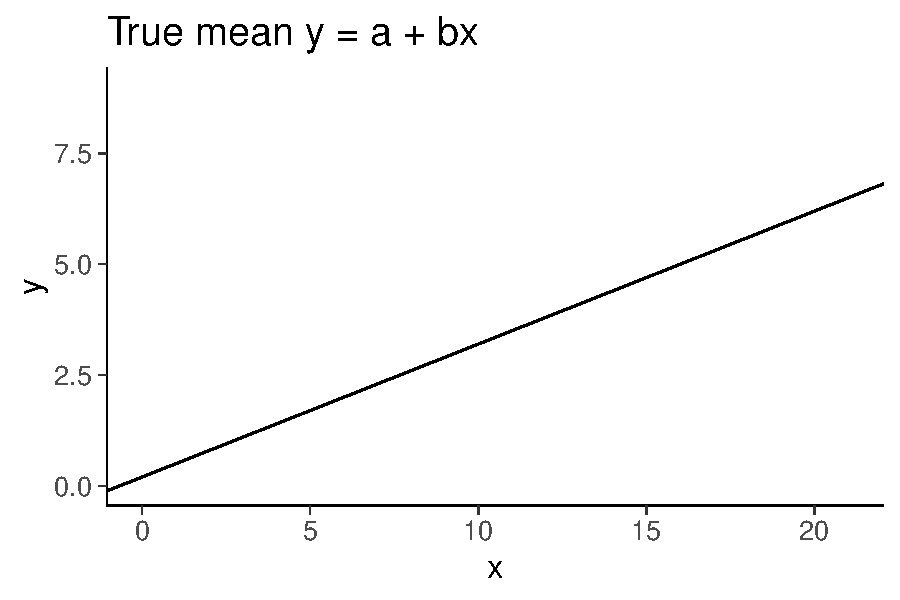
\includegraphics[width=10cm]{fake1.pdf}}
  \only<2>{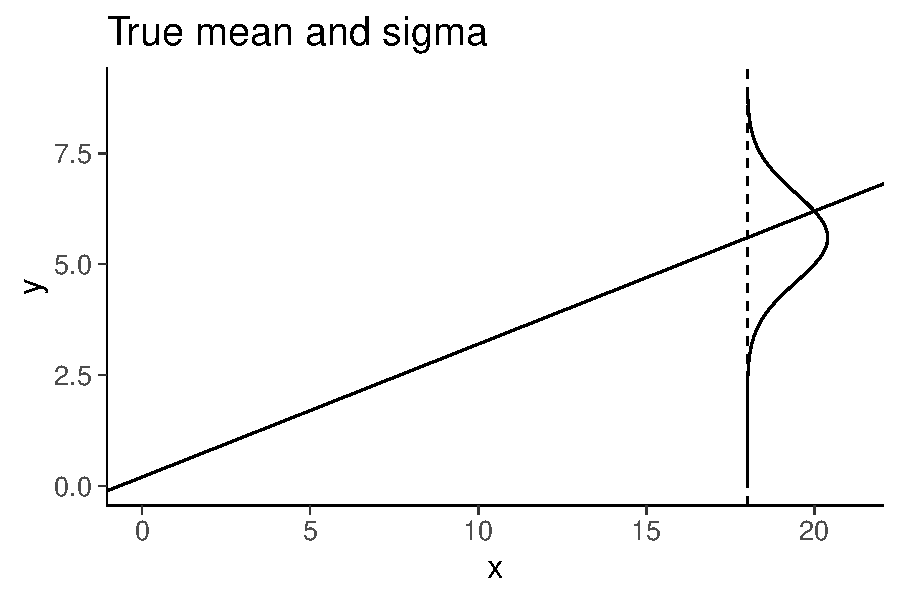
\includegraphics[width=10cm]{fake2.pdf}}
  \only<3>{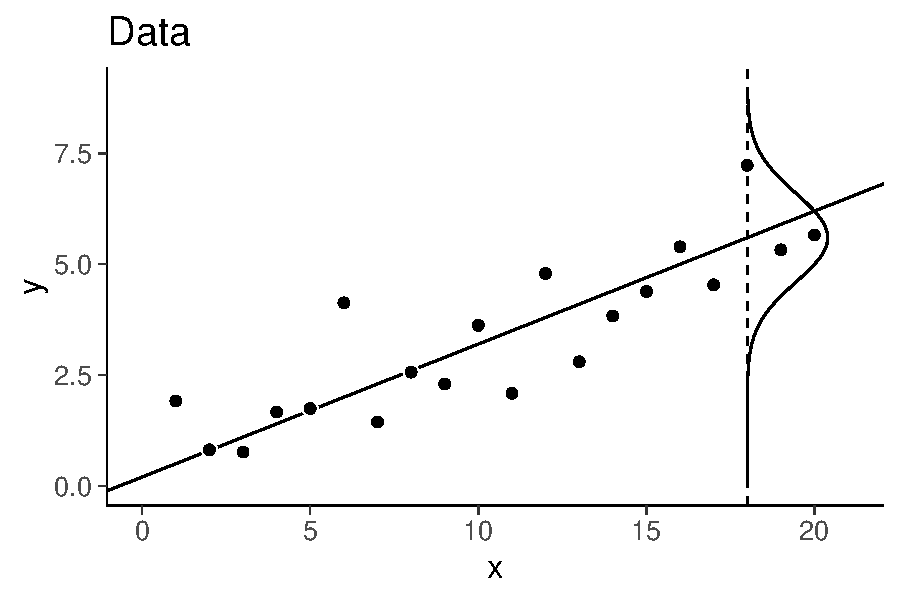
\includegraphics[width=10cm]{fake3.pdf}}
  \only<4>{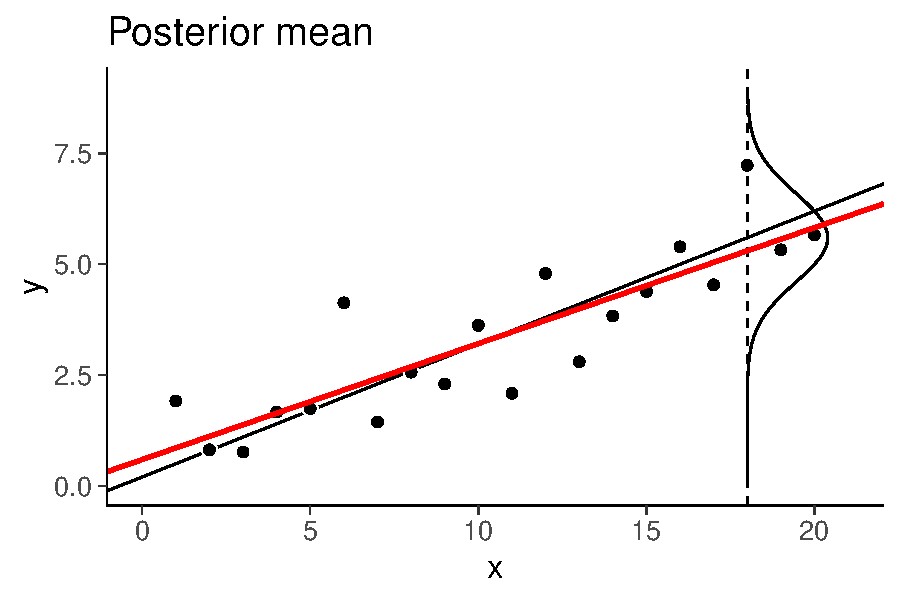
\includegraphics[width=10cm]{fake4.pdf}}
  \only<5>{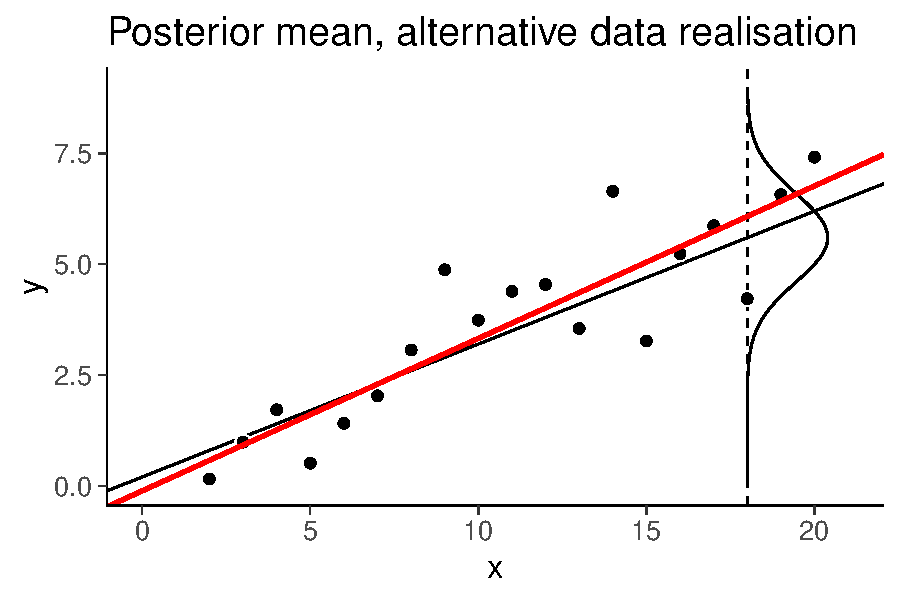
\includegraphics[width=10cm]{fake4b.pdf}}
  \only<6>{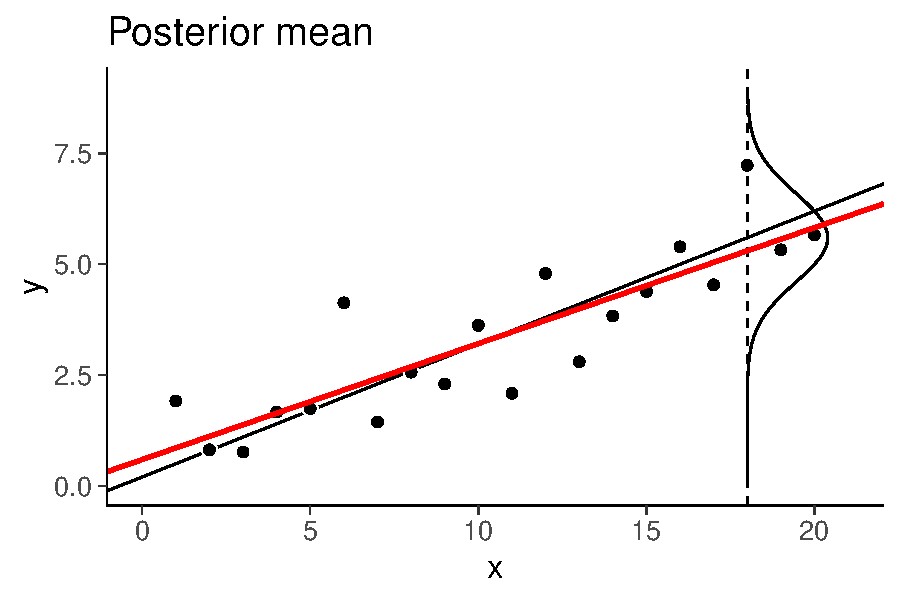
\includegraphics[width=10cm]{fake4.pdf}}
  \only<7>{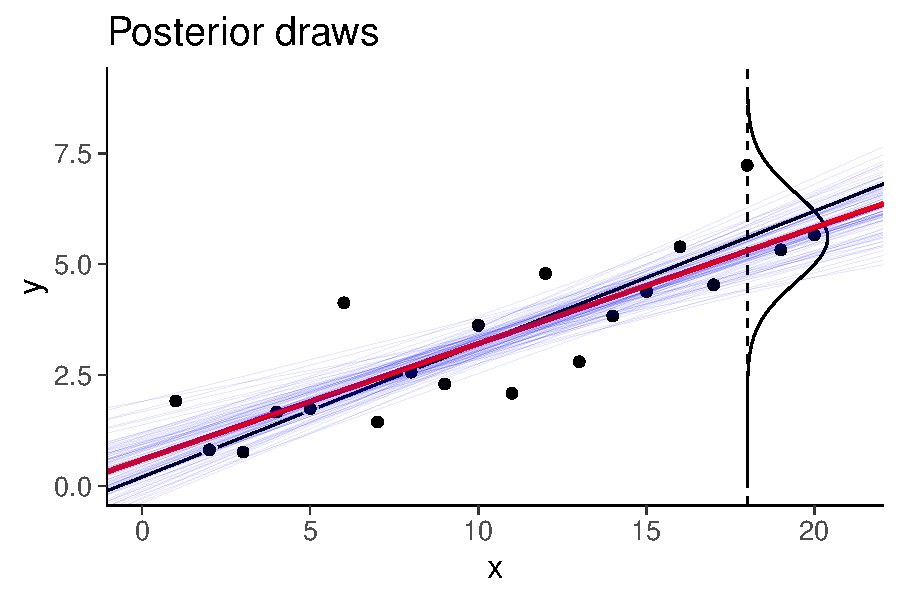
\includegraphics[width=10cm]{fake4s.pdf}}
  \only<8-9>{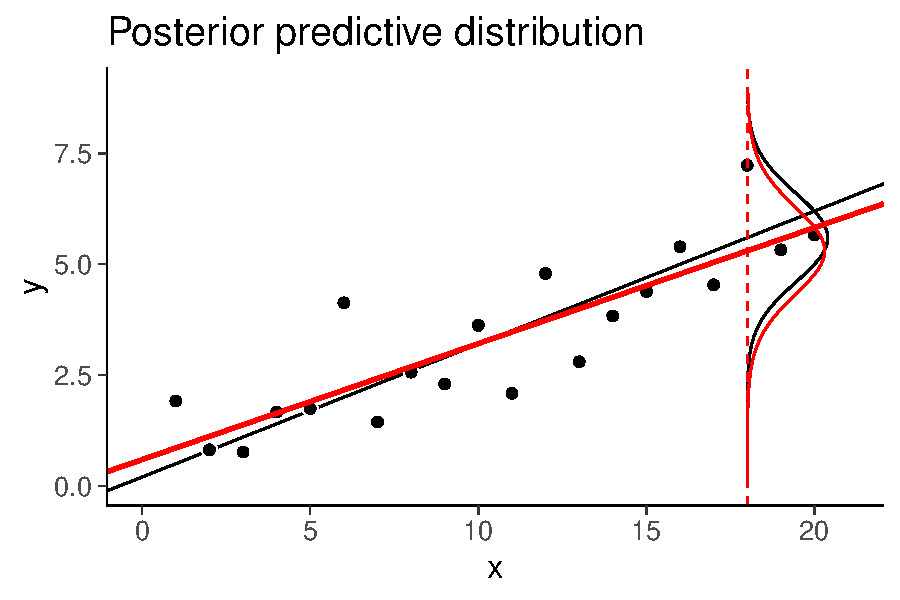
\includegraphics[width=10cm]{fake5.pdf}}
  \only<10>{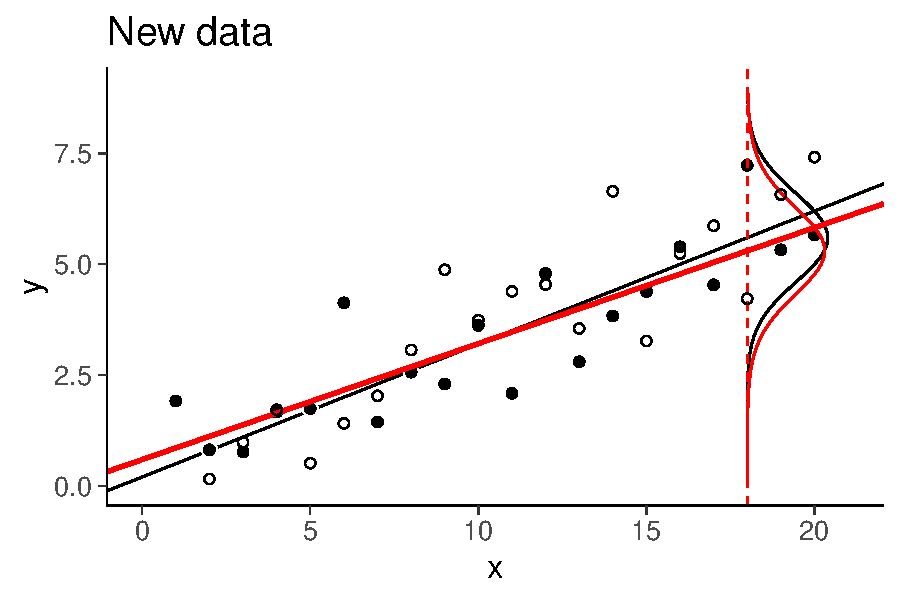
\includegraphics[width=10cm]{fake5n.pdf}}
  \only<11>{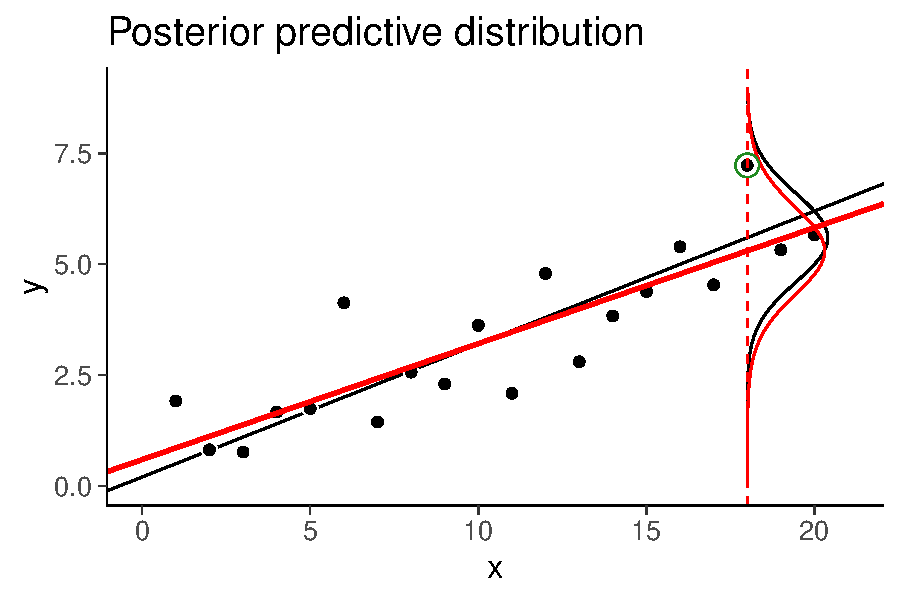
\includegraphics[width=10cm]{fake6.pdf}}
  \only<12>{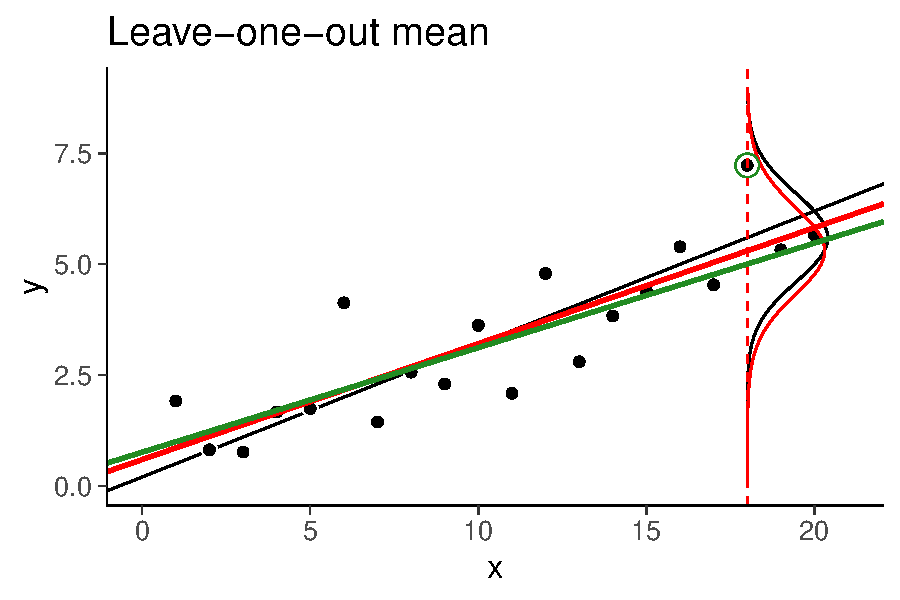
\includegraphics[width=10cm]{fake7.pdf}}
  \\
  \onslide<9>{\color{red} $p(\tilde{y}|\tilde{x}=18,x,y)=\int p(\tilde{y}|\tilde{x}=18,\theta)p(\theta|x,y)d\theta$\\ \vspace{0.5\baselineskip}}
\end{frame}

\begin{frame}{}

  {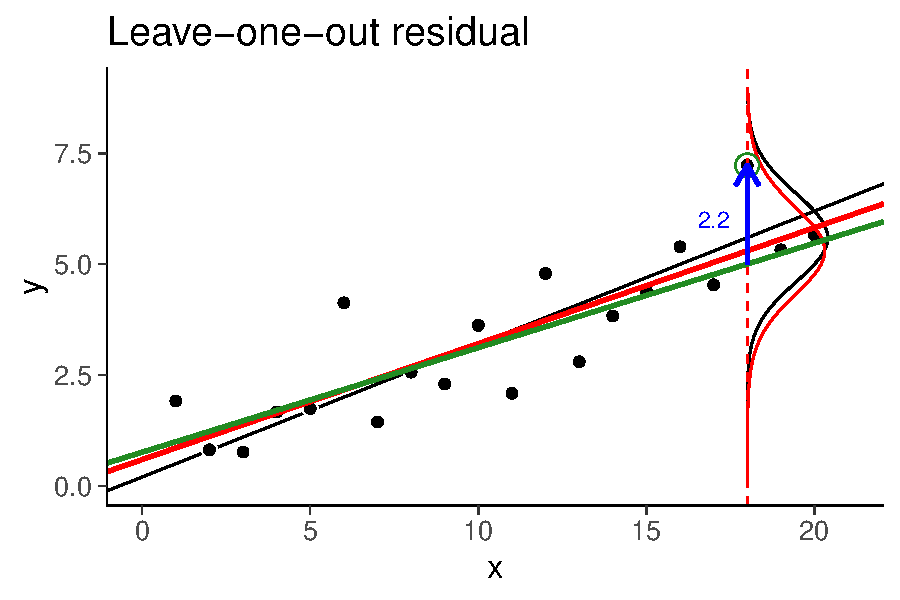
\includegraphics[width=10cm]{fake7r.pdf}}
  \\
  \onslide<2->{{\color{blue} $y_{18} - E[p(\tilde{y}|\tilde{x}=18,x_{-18},y_{-18})]$}\\ \vspace{0.5\baselineskip}}
  \onslide<3->{Can be use to compute, e.g., RMSE, $R^2$, 90\% error}
  \onslide<4>{\\~\\ \small See LOO-$R^2$ at \url{avehtari.github.io/bayes_R2/bayes_R2.html}}
\end{frame}

\begin{frame}{}

  {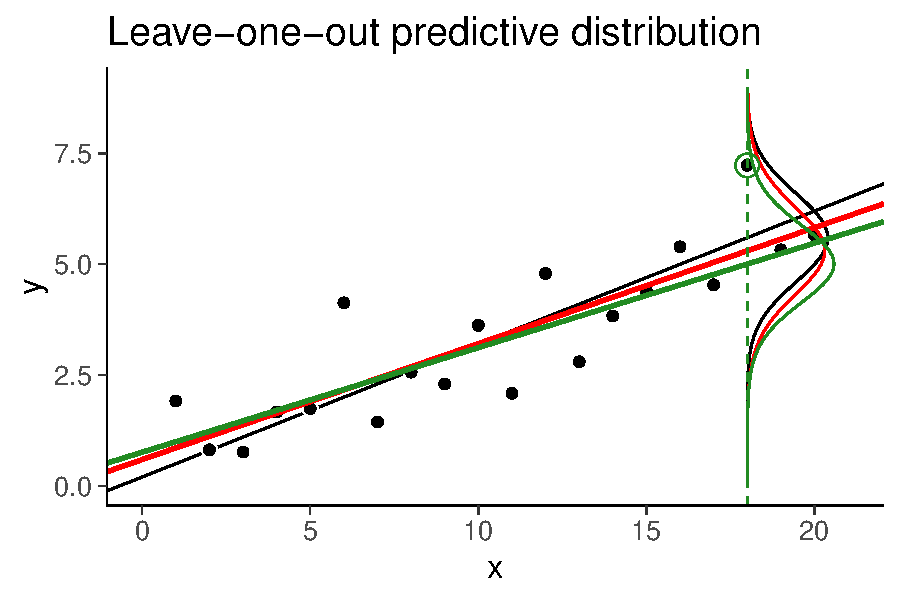
\includegraphics[width=10cm]{fake8.pdf}}
  \\
  \onslide<2>{\color{forestgreen} $p(\tilde{y}|\tilde{x}=18,x_{-18},y_{-18})=\int p(\tilde{y}|\tilde{x}=18,\theta)p(\theta|x_{-18},y_{-18})d\theta$}
  
\end{frame}

\begin{frame}{}

  \only<1-2>{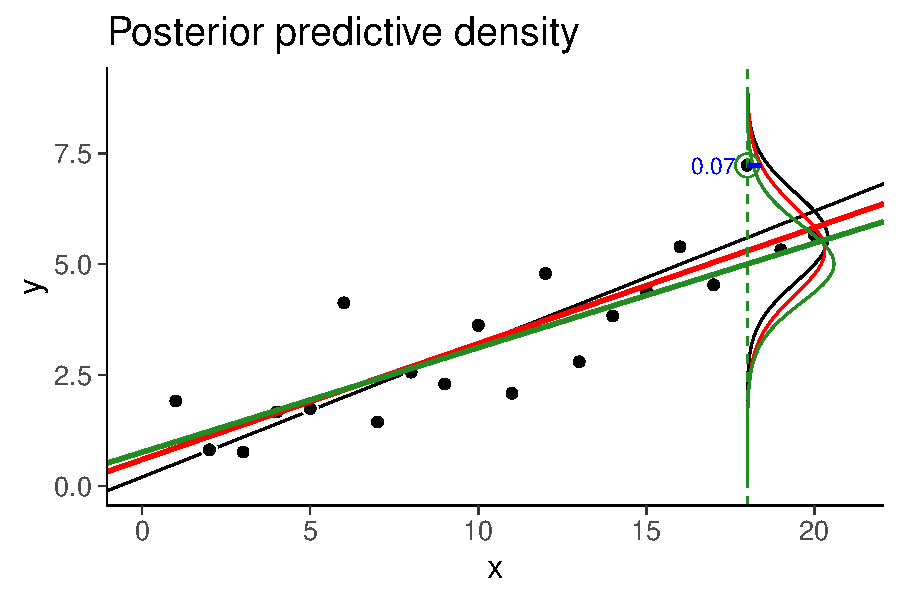
\includegraphics[width=10cm]{fake8pd.pdf}}
  \only<3>{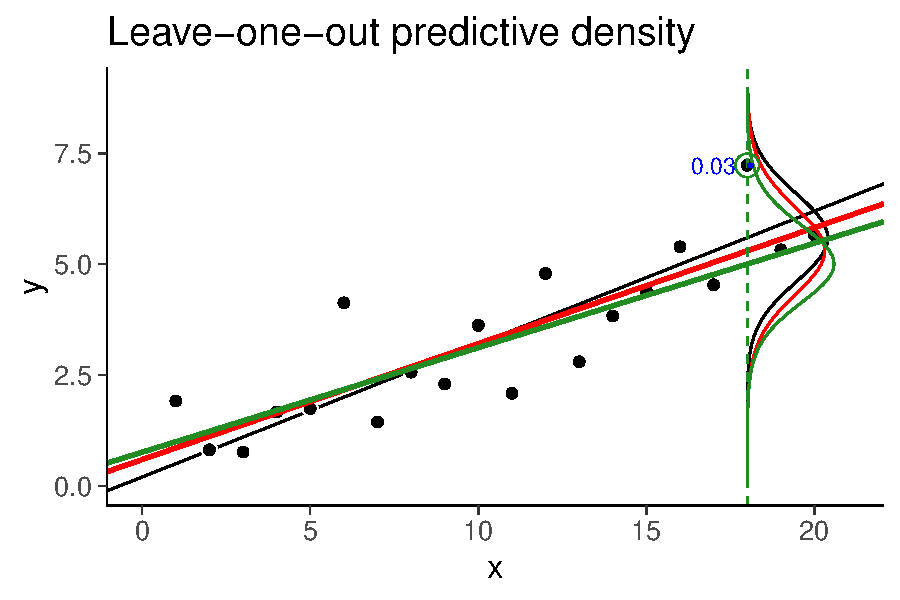
\includegraphics[width=10cm]{fake8loopd.pdf}}
  \\
  \onslide<2->{\color{red} $p(\tilde{y}=y_{18}|\tilde{x}=18,x,y) \approx 0.07$\\ \vspace{0.5\baselineskip}}
  \onslide<3>{\color{forestgreen} $p(\tilde{y}=y_{18}|\tilde{x}=18,x_{-18},y_{-18}) \approx 0.03$}
  
\end{frame}

\begin{frame}{}

  \only<1>{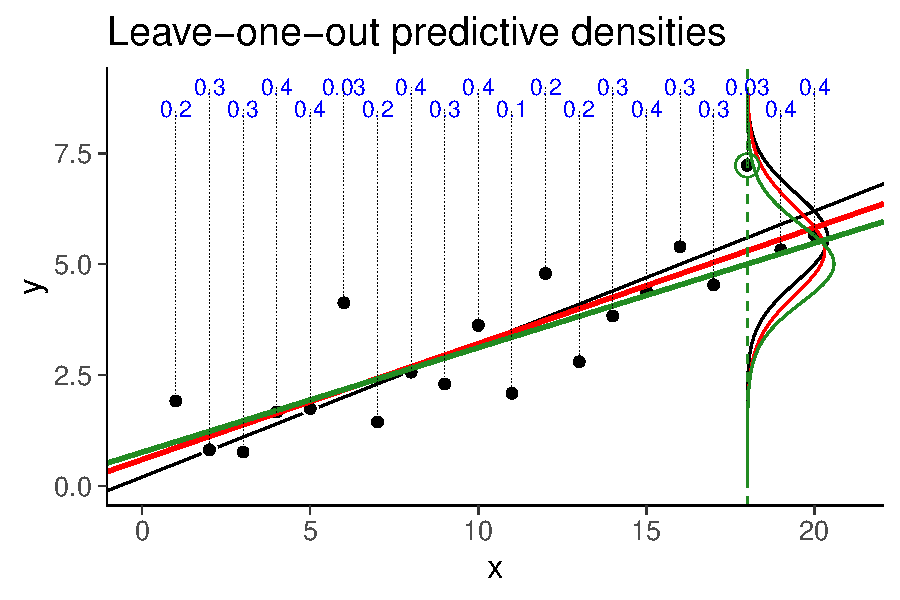
\includegraphics[width=10cm]{fake8loopds.pdf}}
  \only<2->{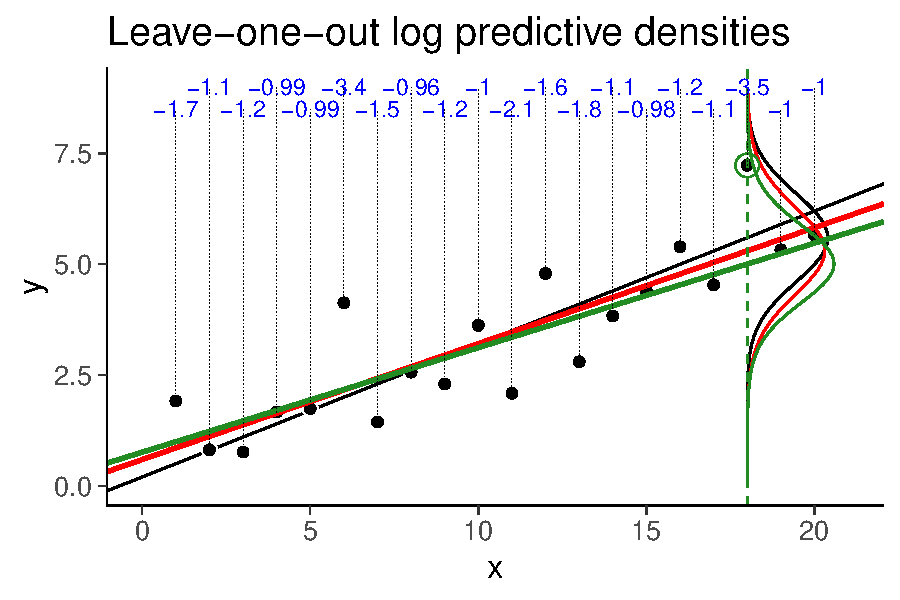
\includegraphics[width=10cm]{fake8loolpds.pdf}}
  \\ \vspace{-0.5\baselineskip}
  \only<1>{\color{blue} $p(y_i|x_i,x_{-i},y_{-i}), \quad i=1,\ldots,20$}
  \only<2>{\color{blue} $\log p(y_i|x_i,x_{-i},y_{-i}), \quad i=1,\ldots,20$}
  \only<3>{\color{blue} $\sum_{i=1}^{20} \log p(y_i|x_i,x_{-i},y_{-i}) \approx -29.5$}
  \only<4->{\color{blue} $\mbox{elpd\_loo} = \sum_{i=1}^{20} \log p(y_i|x_i,x_{-i},y_{-i}) \approx -29.5$\\ \vspace{0.2\baselineskip}}
  \only<5> {\color{blue} unbiased estimate of log posterior pred. density for new data}
  \only<6-7>{\color{red} $\mbox{lpd} = \sum_{i=1}^{20} \log p(y_i|x_i,x,y) \approx -26.8$\\ \vspace{0.2\baselineskip}}
  \only<7>{\color{blue} $\mbox{p\_loo} = \mbox{lpd}-\mbox{elpd\_loo} \approx 2.7$}
  \only<8-> {\color{blue} $\mbox{SE} = \mbox{sd}(\log p(y_i|x_i,x_{-i},y_{-i}))\cdot \sqrt{20} \approx 3.3$}
  \only<9>{\\~\\~\\ \color{black} \footnotesize see \href{http://link.springer.com/article/10.1007/s11222-016-9696-4}{Vehtari, Gelman \& Gabry (2017a)} and \href{http://dx.doi.org/10.1214/12-SS102}{Vehtari \& Ojanen (2012)} for more}
  
\end{frame}

\begin{frame}{}

  \only<1>{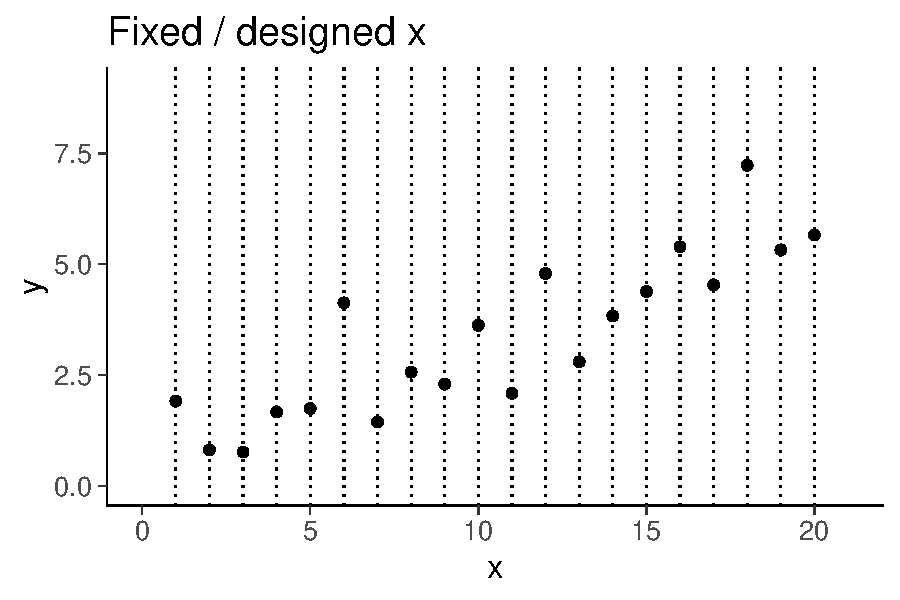
\includegraphics[width=10cm]{fakedfixed.pdf}}
  \only<2->{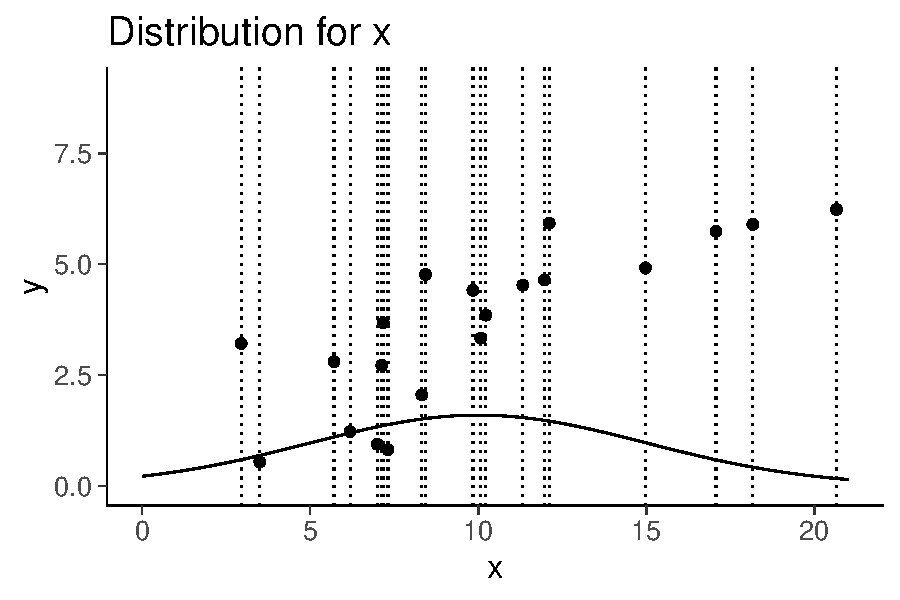
\includegraphics[width=10cm]{fakedrandom.pdf}}
  \\ \vspace{-0.5\baselineskip}
  \only<1>{LOO is ok for fixed / designed $x$. SE is uncertainty about $y|x$.\\ \vspace{0.2\baselineskip}}
  \only<2->{LOO is ok for random $x$. SE is uncertainty about $y|x$ and $x$.\\ \vspace{0.2\baselineskip}}
  \onslide<3>{Covariate shift can be handled with importance weighting or modelling}
  \onslide<1->{\\ \small see \href{http://dx.doi.org/10.1214/12-SS102}{Vehtari \& Ojanen (2012)} and \url{andrewgelman.com/2018/08/03/loo-cross-validation-approaches-valid/}}
  
\end{frame}

\begin{frame}[fragile]

  {\Large\color{navyblue} {\tt loo} package}

  {\scriptsize
\begin{lstlisting}
 Computed from 4000 by 20 log-likelihood matrix

         Estimate  SE
elpd_loo    -29.5 3.3
p_loo         2.7 1.0
\end{lstlisting}
      {\color{gray}
\begin{lstlisting}
------
Monte Carlo SE of elpd_loo is 0.1.

Pareto k diagnostic values:
                         Count Pct.    Min. n_eff
(-Inf, 0.5]   (good)     18    90.0%   899       
 (0.5, 0.7]   (ok)        2    10.0%   459       
   (0.7, 1]   (bad)       0     0.0%   <NA>      
   (1, Inf)   (very bad)  0     0.0%   <NA>      

All Pareto k estimates are ok (k < 0.7).
See help('pareto-k-diagnostic') for details.
\end{lstlisting}}
}
\end{frame}

\begin{frame}{}

  \only<1>{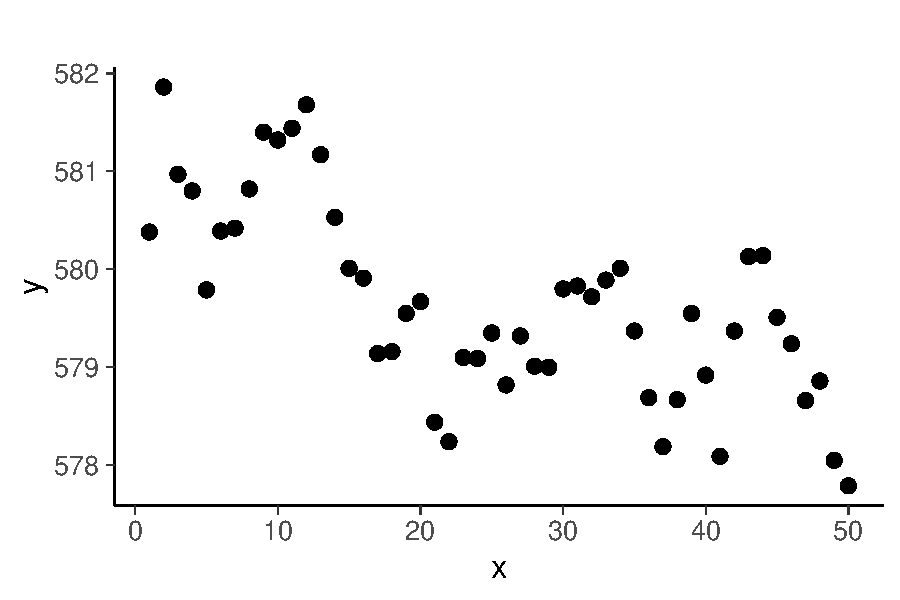
\includegraphics[width=10cm]{lake1data.pdf}}
  \only<2>{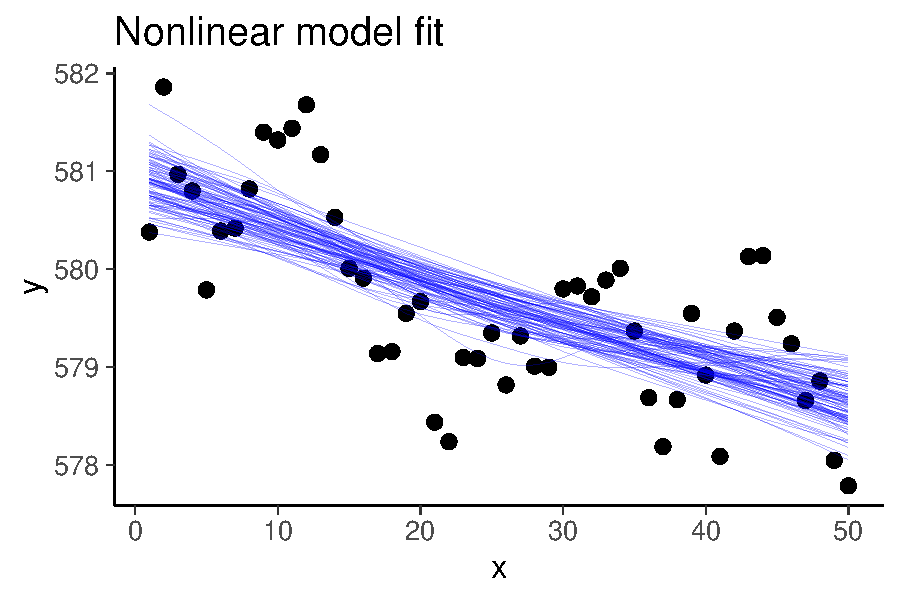
\includegraphics[width=10cm]{lake1gp.pdf}}
  \only<3->{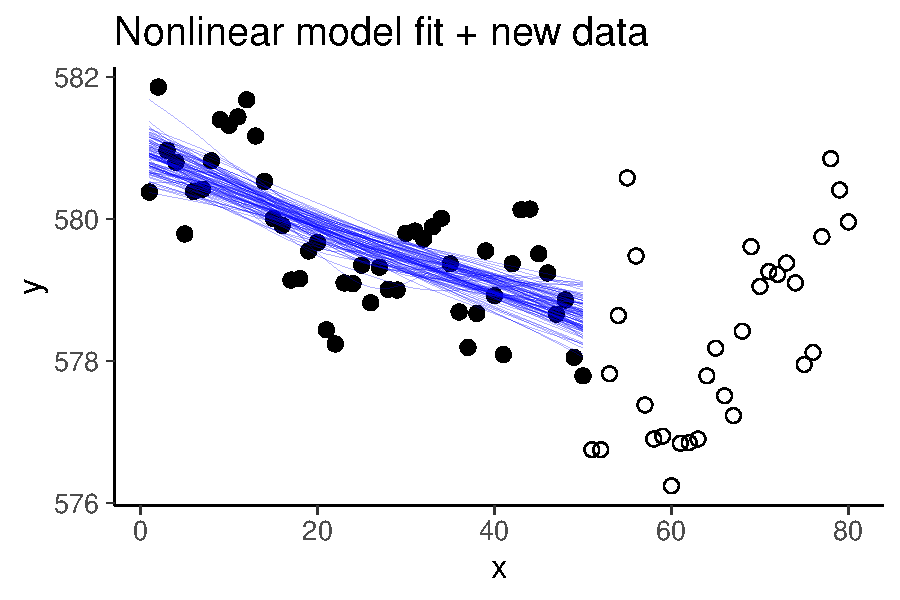
\includegraphics[width=10cm]{lake1gpptest.pdf}}
  \\
  \only<4>{Extrapolation is more difficult}
  
\end{frame}

\begin{frame}{}

  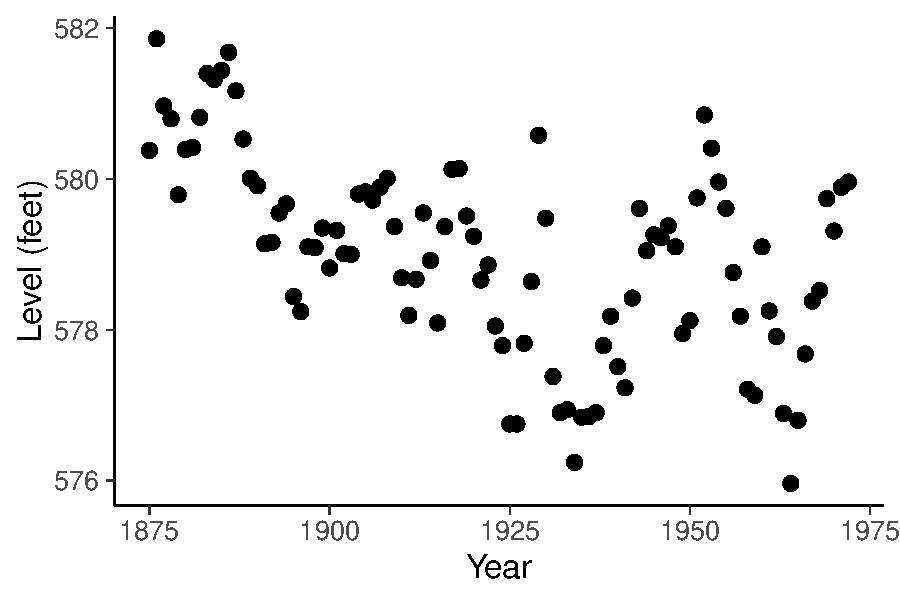
\includegraphics[width=10cm]{lake2data.pdf}

  
  {Can LOO or other cross-validation be used with time series?}
  
\end{frame}

\begin{frame}{}

  \only<1>{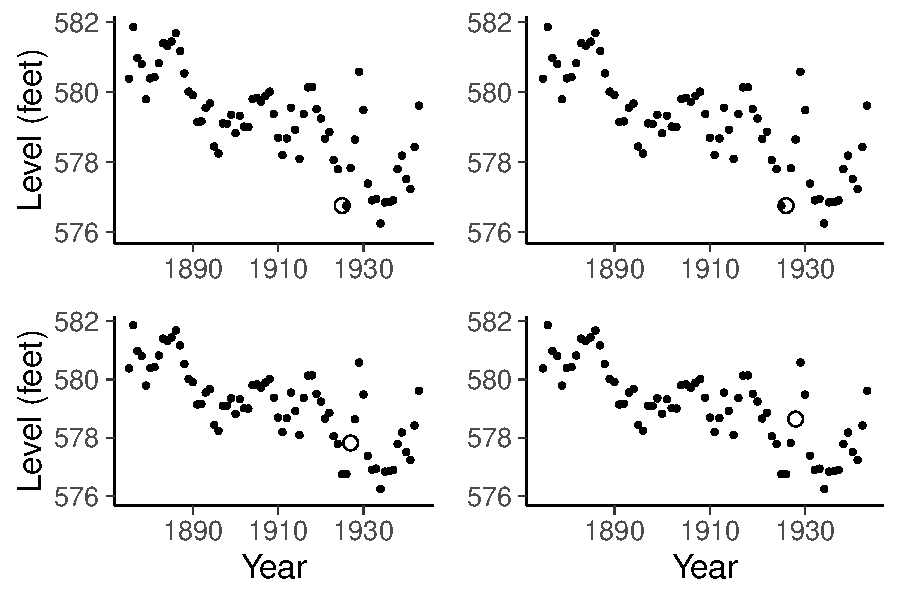
\includegraphics[width=10cm]{lake3loo.pdf}}
  \only<2>{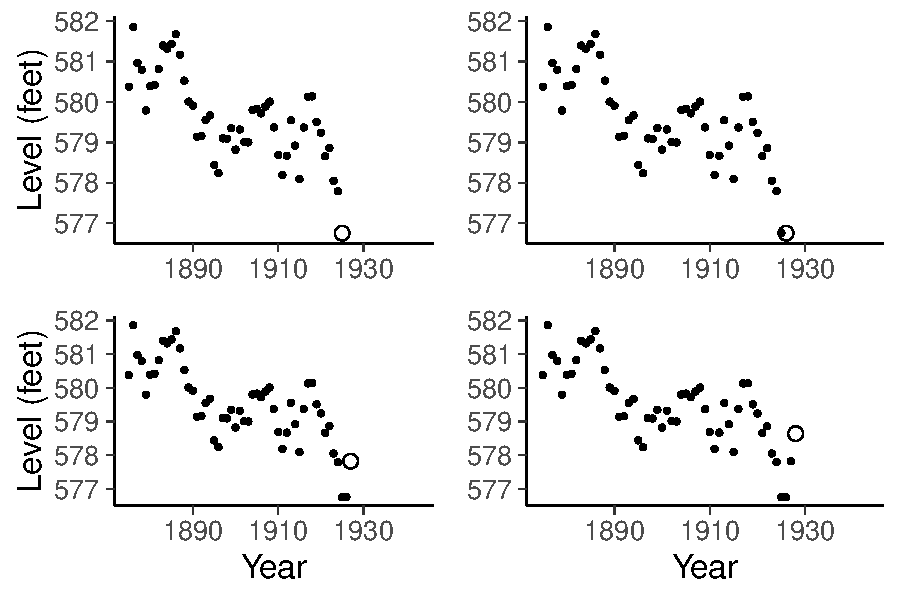
\includegraphics[width=10cm]{lake3stepahead.pdf}}
  \only<3>{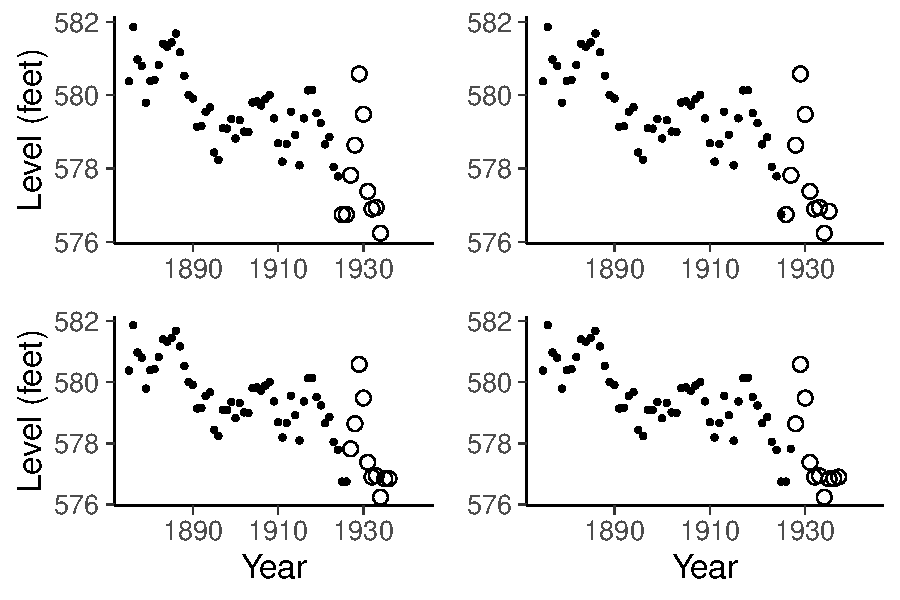
\includegraphics[width=10cm]{lake3tenstepahead.pdf}}
  \only<4>{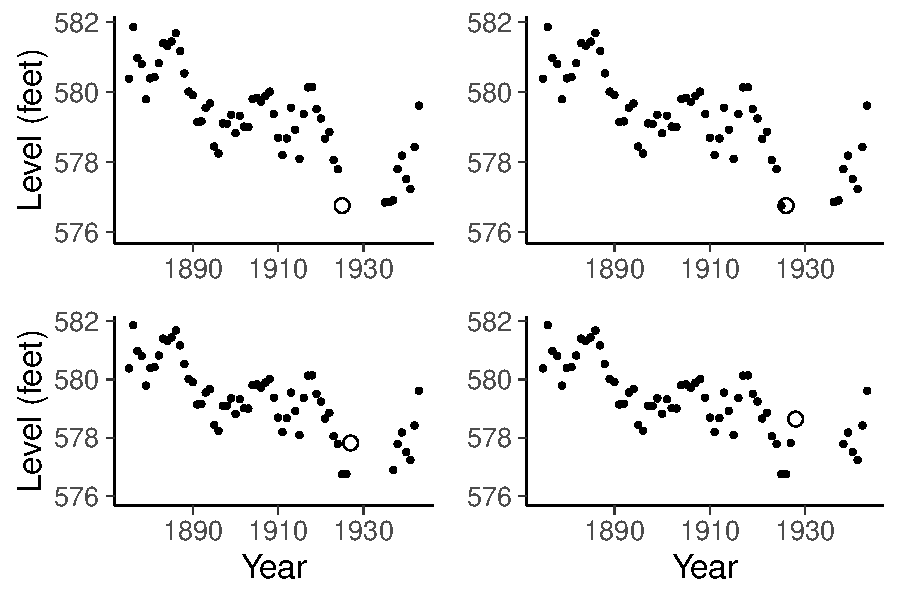
\includegraphics[width=10cm]{lake3stepaheadblock.pdf}}
  \\
  \only<1>{Leave-one-out cross-validation is ok for assessing conditional model}
  \only<2>{Leave-future-out cross-validation is better for predicting future}
  \only<3>{$m$-step-ahead cross-validation is better for predicting further future}
  \only<4>{$m$-step-ahead leave-a-block-out cross-validation}
  
\end{frame}

\begin{frame}{}

  \only<1>{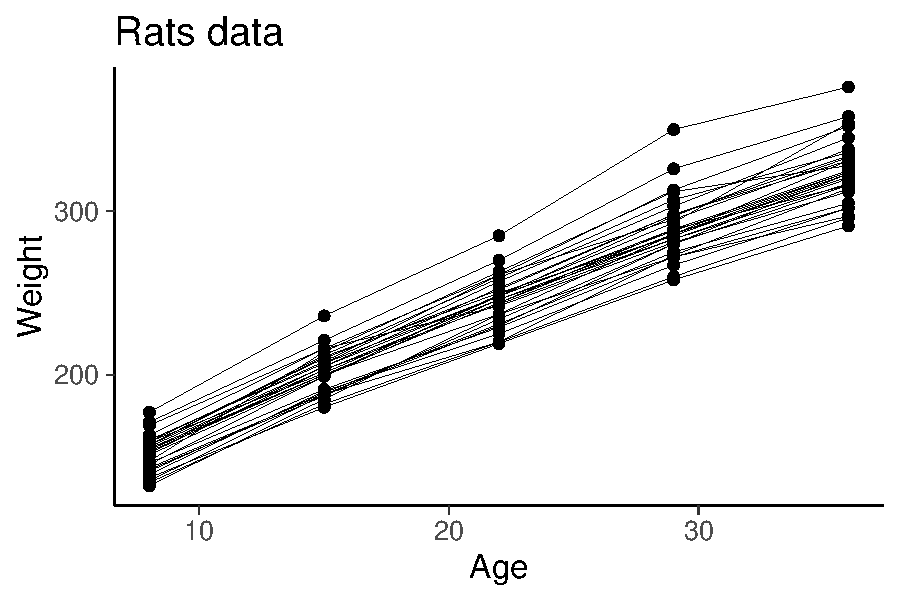
\includegraphics[width=10cm]{rats1data.pdf}}
  \only<2>{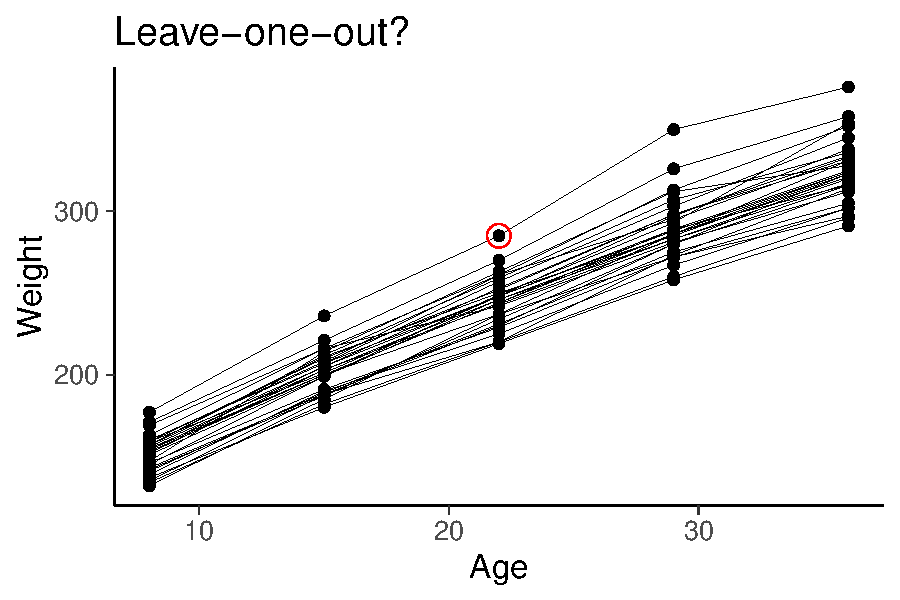
\includegraphics[width=10cm]{rats1loo.pdf}}
  \only<3>{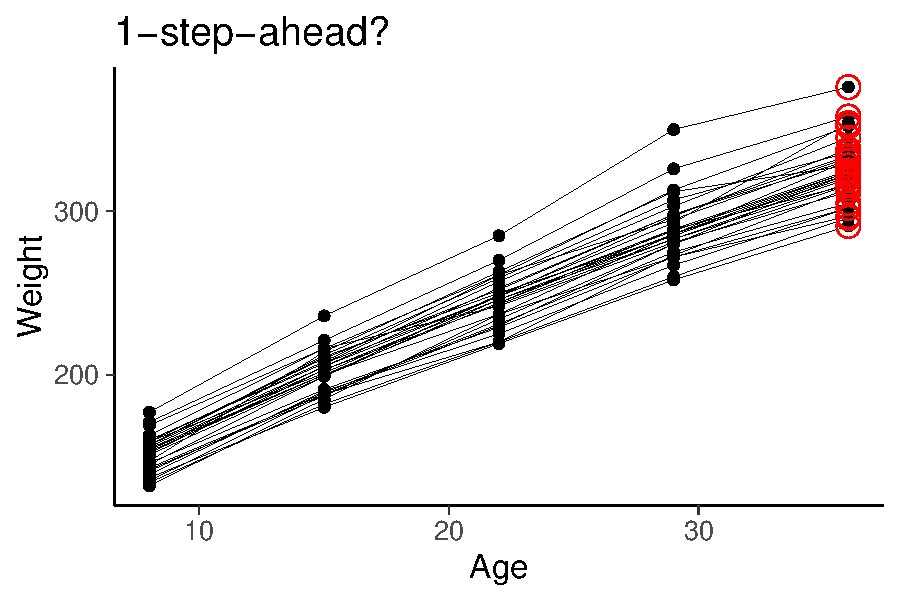
\includegraphics[width=10cm]{rats1step.pdf}}
  \only<4>{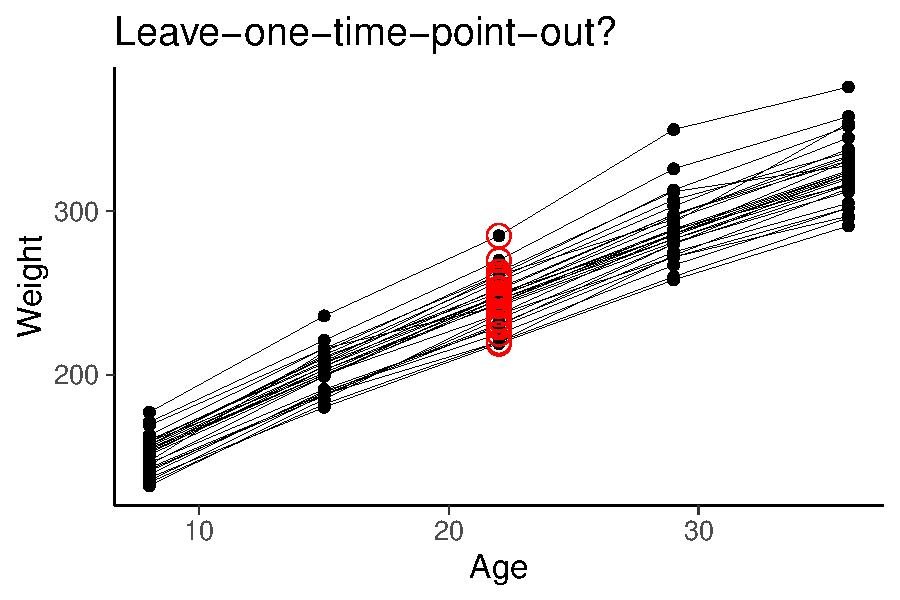
\includegraphics[width=10cm]{rats1onetime.pdf}}
  \only<5>{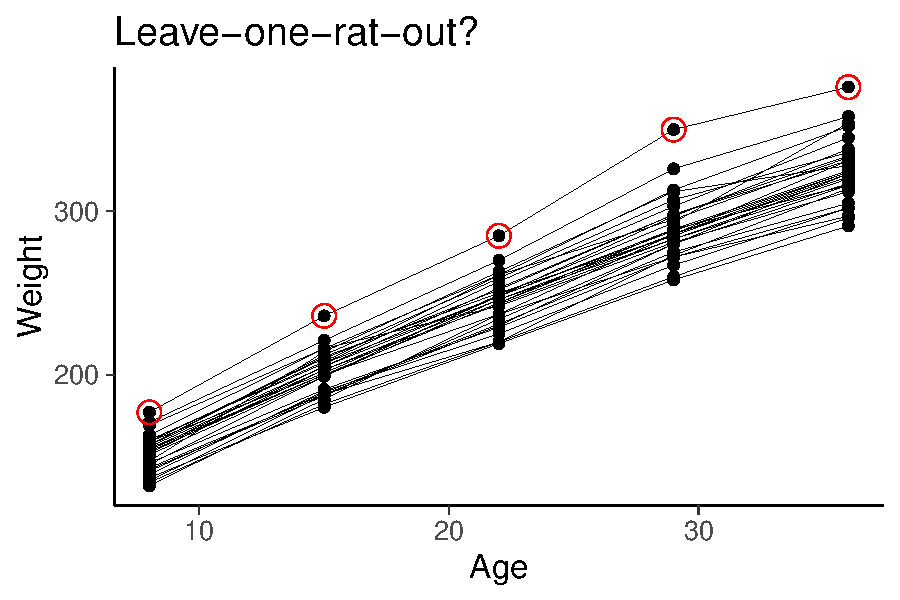
\includegraphics[width=10cm]{rats1onerat.pdf}}
  \only<6>{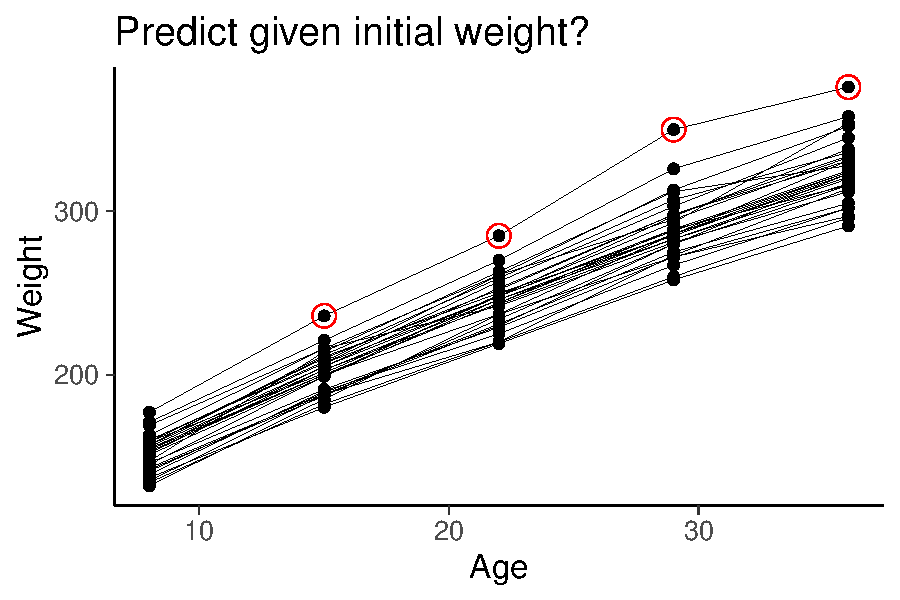
\includegraphics[width=10cm]{rats1init.pdf}}
  \\
  \only<1>{Can LOO or other cross-validation be used with hierarchical data?}
  \only<2->{Yes!}
  
\end{frame}

\begin{frame}{}

{\Large\color{navyblue} Summary of data generating mechanisms and prediction tasks}

\begin{list1}
\item You have to make some assumptions on data generating mechanism
\item Use the knowledge of the prediction task if available
\item Cross-validation can be used to analyse different parts, even if
  there is no clear prediction task
\end{list1}

 \vspace{6.5\baselineskip}
{ \small see \href{http://dx.doi.org/10.1214/12-SS102}{Vehtari \& Ojanen (2012)} and \url{andrewgelman.com/2018/08/03/loo-cross-validation-approaches-valid/}}

\end{frame}

\begin{frame}{}

{\Large\color{navyblue} Fast cross-validation}

\begin{list1}
\item Pareto smoothed importance sampling LOO (PSIS-LOO)
\item K-fold cross-validation
\end{list1}

\vspace{12\baselineskip}

{\small see \href{http://link.springer.com/article/10.1007/s11222-016-9696-4}{Vehtari, Gelman \& Gabry (2017a)} and \url{mc-stan.org/loo/}}

\end{frame}

\begin{frame}{}

  \only<1>{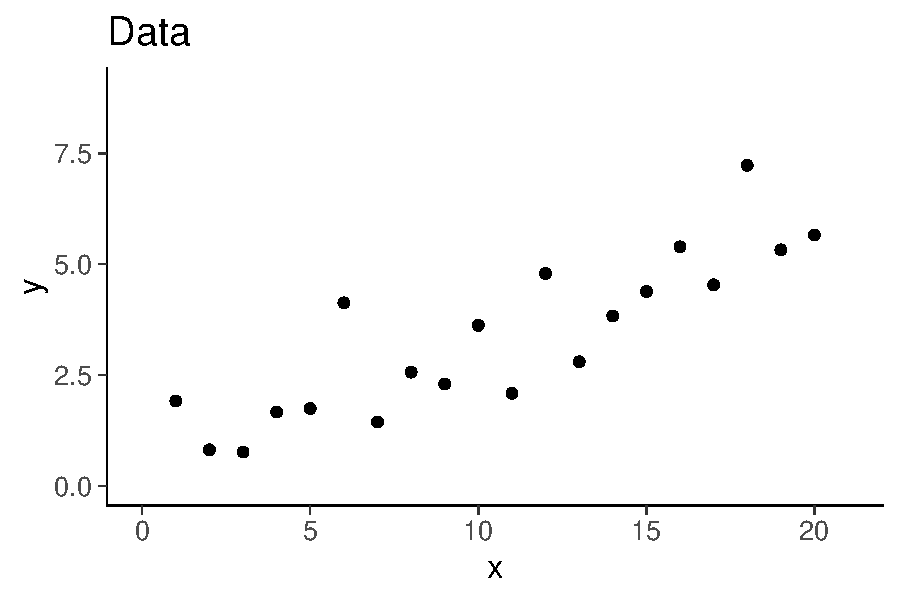
\includegraphics[width=10cm]{fakedata.pdf}}
  \only<2>{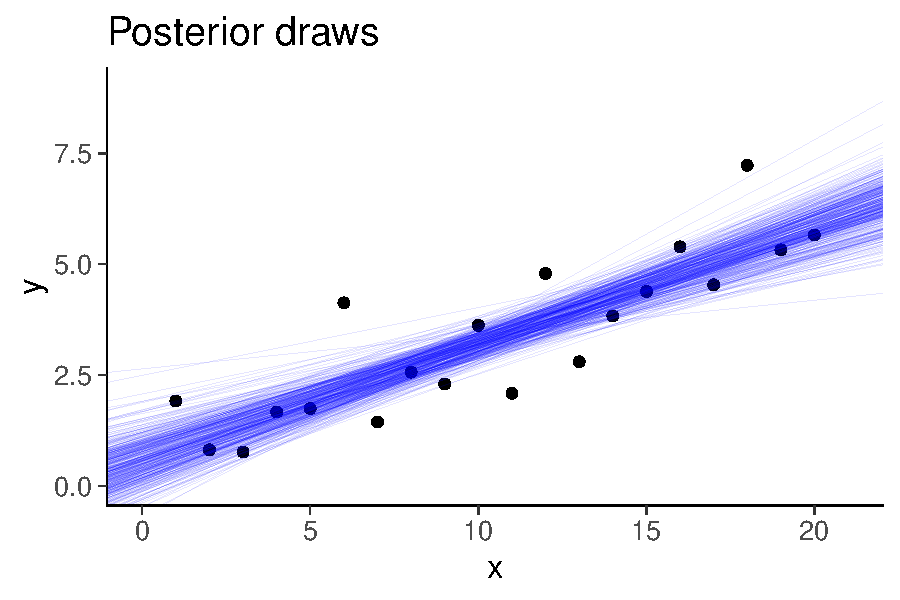
\includegraphics[width=10cm]{fakedraws.pdf}}
  \only<3>{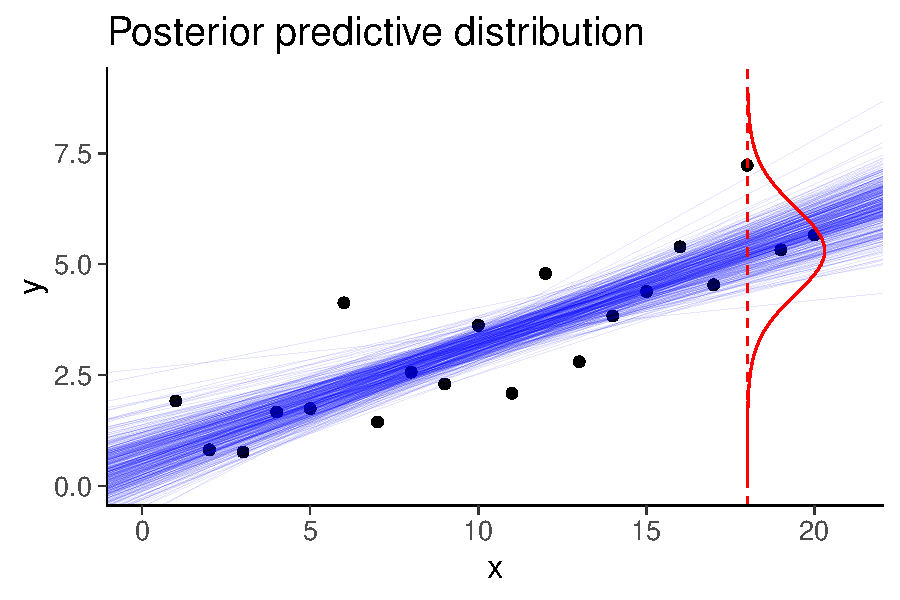
\includegraphics[width=10cm]{fakepostpred.pdf}}
  \only<4>{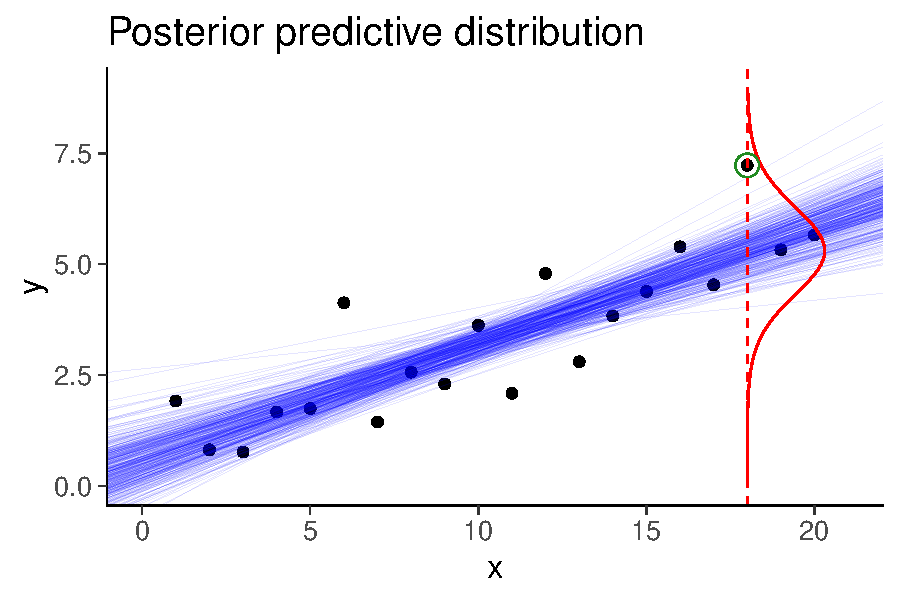
\includegraphics[width=10cm]{fakepostpred18.pdf}}
  \only<5-7>{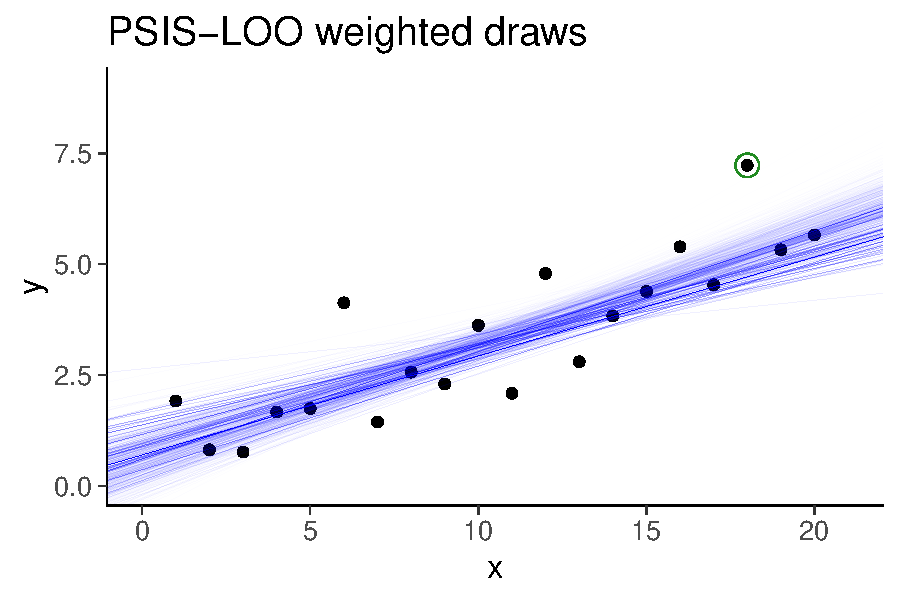
\includegraphics[width=10cm]{fakepsisdraws.pdf}}
  \only<8-10>{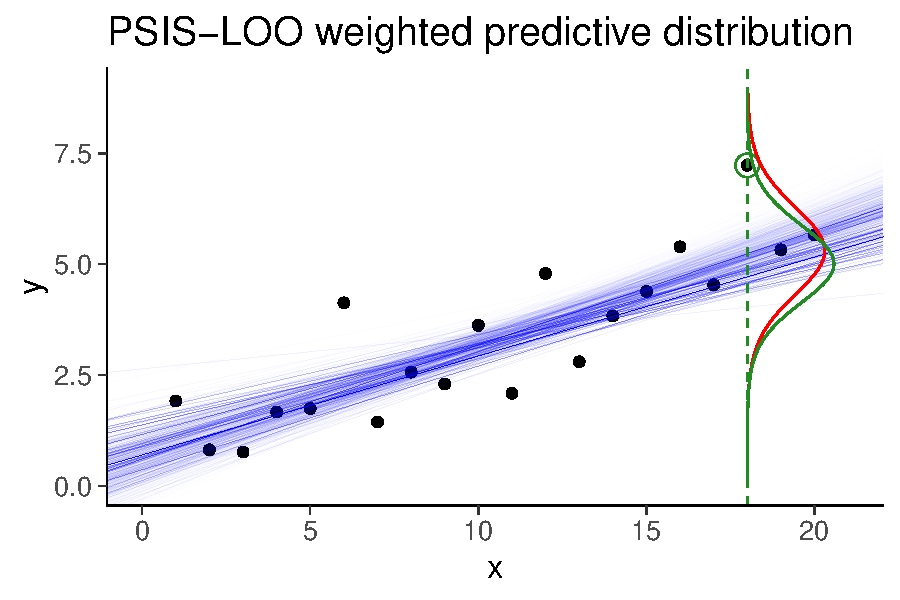
\includegraphics[width=10cm]{fakepsispostpred.pdf}}
  \\
  \only<2>{$\theta^{(s)} \sim p(\theta|x,y)$}
  \only<3-4>{$\theta^{(s)} \sim p(\theta|x,y), \quad p(\tilde{y}|\tilde{x},x,y) \approx \frac{1}{S}\sum_{s=1}^S p(\tilde{y}|\tilde{x},\theta^{(s)})$ }
  \only<5>{$\theta^{(s)} \sim p(\theta|x,y)$\\ \vspace{0.2\baselineskip}$ r_i^{(s)} = p(\theta^{(s)}|x_{-i},y_{-i}) / p(\theta^{(s)}|x,y)$ }
  \only<6-8>{$\theta^{(s)} \sim p(\theta|x,y)$\\ \vspace{0.2\baselineskip} $ r_i^{(s)} = p(\theta^{(s)}|x_{-i},y_{-i}) / p(\theta^{(s)}|x,y) \propto 1/p(y_i|x_i,\theta^{(s)})$\\ \vspace{0.2\baselineskip} }
  \only<7>{$\log(1/p(y_i|x_i,\theta^{(s)})) = -\mbox{log\_lik}[i]$}
  \only<9-10>{$\theta^{(s)} \sim p(\theta|x,y)$\\ \vspace{0.2\baselineskip}
    $ r_i^{(s)} = p(\theta^{(s)}|x_{-i},y_{-i}) / p(\theta^{(s)}|x,y) \propto 1/p(y_i|x_i,\theta^{(s)})$\\ \vspace{0.2\baselineskip}
  $p(y_i|x_i,x_{-i},y_{-i}) \approx \sum_{s=1}^S [w_i^{(s)} p(y_i|x_i,\theta^{(s)})]$}\only<10>{, where $w \leftarrow \mbox{PSIS}(r)$}
  
\end{frame}

\begin{frame}{}

  \only<1>{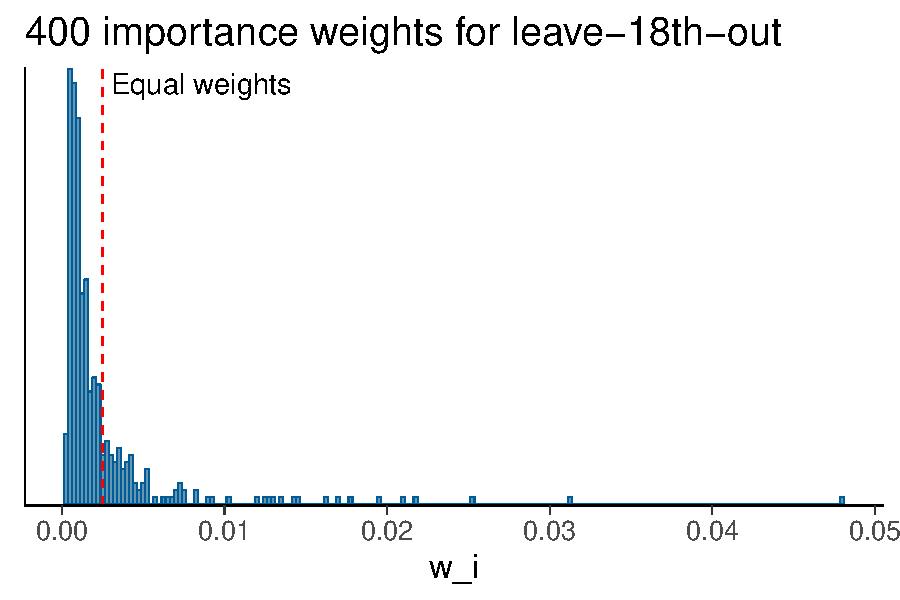
\includegraphics[width=10cm]{fakepsisweights.pdf}}
  \only<2->{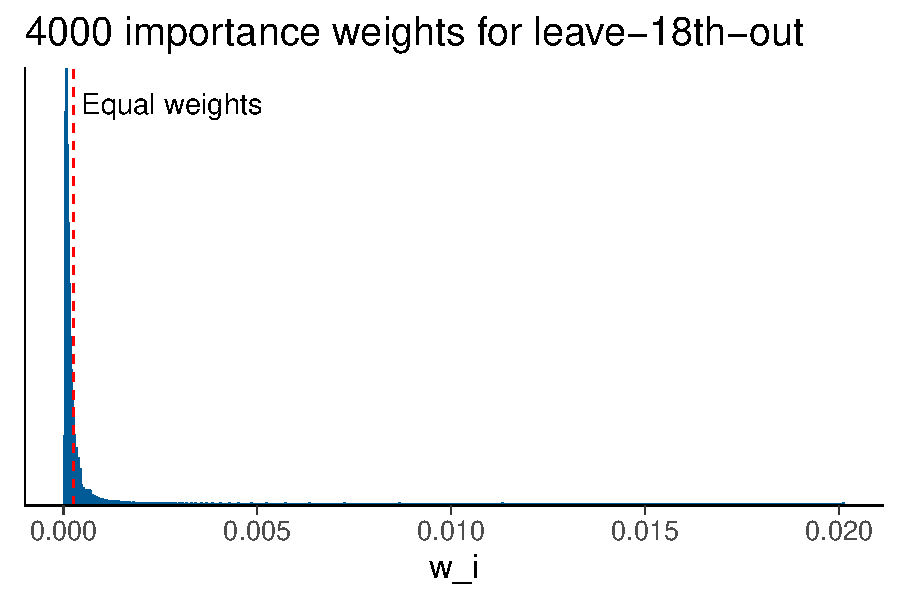
\includegraphics[width=10cm]{fakepsisweights4000.pdf}}
  \\
  \vspace{-\baselineskip}
  \onslide<3->{n\_eff $\approx$ 459\\  \vspace{0.2\baselineskip}}
  \onslide<4>{Pareto $\hat{k}$ $\approx$ 0.52
  \vspace{-\parskip}
    \begin{list2}
    \item Pareto $\hat{k}$ estimates the tail shape which determines the convergence rate of PSIS. Less than 0.7 is ok.}
\end{list2}
  \onslide<3->{\vspace{0.1\baselineskip}\small see \href{http://link.springer.com/article/10.1007/s11222-016-9696-4}{Vehtari, Gelman \& Gabry (2017b)}}
\end{frame}

\begin{frame}[fragile]

  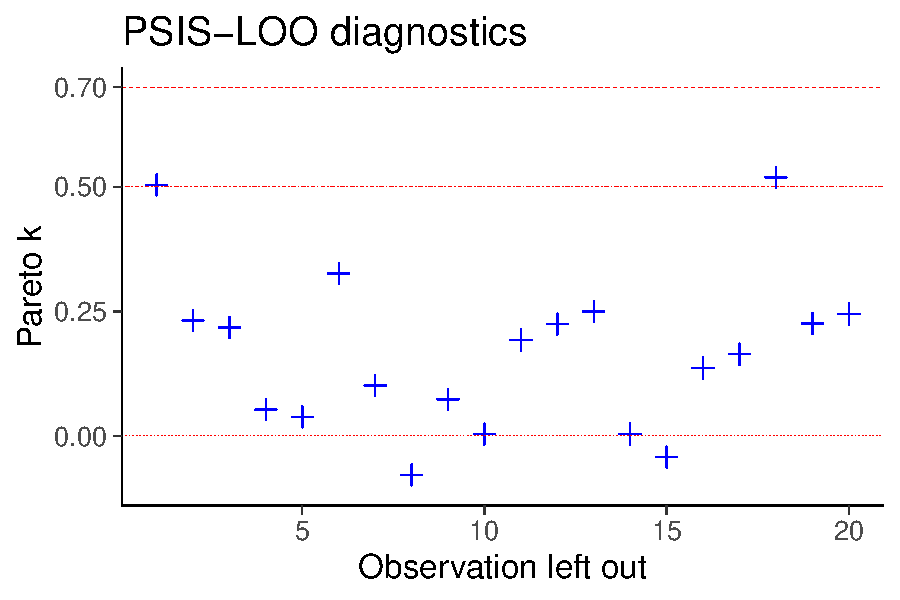
\includegraphics[width=10cm]{fakepks.pdf}

\end{frame}

\begin{frame}[fragile]

  \only<1>{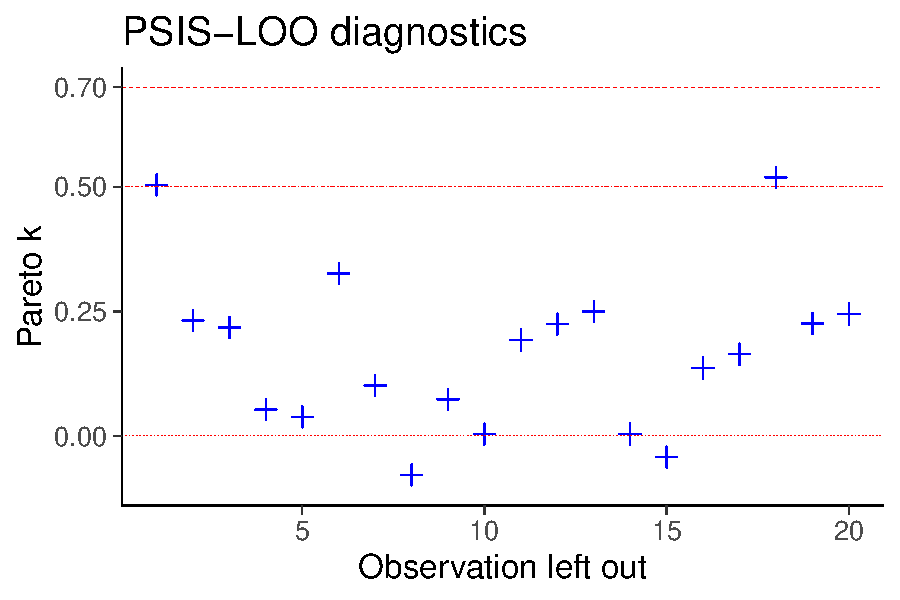
\includegraphics[width=10cm]{fakepks.pdf}}
  \only<2>{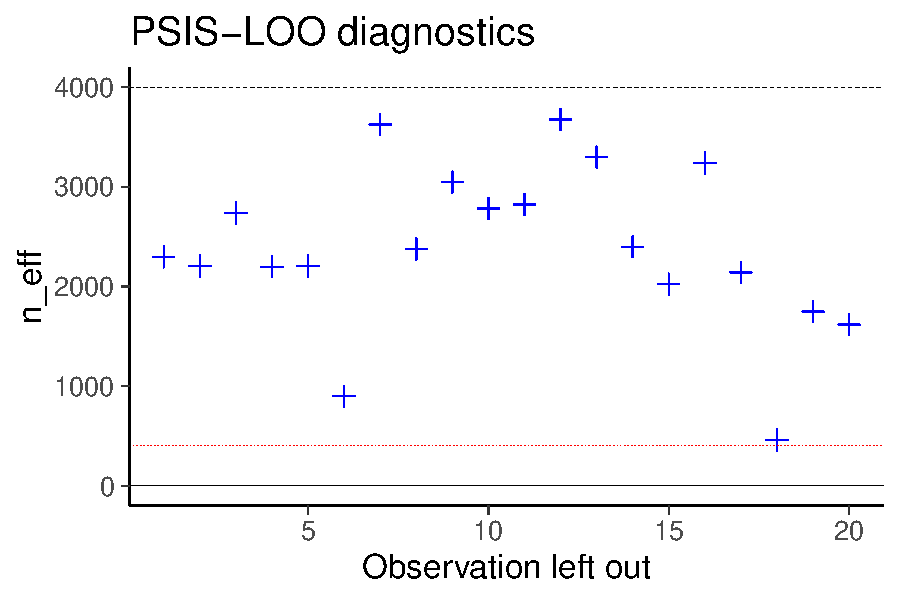
\includegraphics[width=10cm]{fakeneffs.pdf}}
  \\
  {\scriptsize
\begin{lstlisting}
    Pareto k diagnostic values:
                         Count Pct.    Min. n_eff
(-Inf, 0.5]   (good)     18    90.0%   899       
 (0.5, 0.7]   (ok)        2    10.0%   459       
   (0.7, 1]   (bad)       0     0.0%   <NA>      
   (1, Inf)   (very bad)  0     0.0%   <NA>      
\end{lstlisting}
}

\end{frame}

\begin{frame}[fragile]

  {\Large\color{navyblue} {\tt loo} package}

  {\scriptsize
    {\color{gray}
\begin{lstlisting}
 Computed from 4000 by 20 log-likelihood matrix

         Estimate  SE
elpd_loo    -29.5 3.3
p_loo         2.7 1.0
\end{lstlisting}
      }
\begin{lstlisting}
------
Monte Carlo SE of elpd_loo is 0.1.

Pareto k diagnostic values:
                         Count Pct.    Min. n_eff
(-Inf, 0.5]   (good)     18    90.0%   899       
 (0.5, 0.7]   (ok)        2    10.0%   459       
   (0.7, 1]   (bad)       0     0.0%   <NA>      
   (1, Inf)   (very bad)  0     0.0%   <NA>      

All Pareto k estimates are ok (k < 0.7).
See help('pareto-k-diagnostic') for details.
\end{lstlisting}
    }

    {\vspace{2\baselineskip}\small see more in \href{http://link.springer.com/article/10.1007/s11222-016-9696-4}{Vehtari, Gelman \& Gabry (2017b)}}

\end{frame}

% \begin{frame}
%   \frametitle{Importance sampling}

%   \begin{itemize}
%   \item Having samples $\theta^s$ from $p(\theta^s|D)$
%     \begin{align*}
%       p(\tilde{y}_i|x_i,D_{-i})\approx\frac{\sum_{s=1}^Sp(\tilde{y}_i|\theta^s)w_i^s}{\sum_{s=1}^S w_i^s},
%     \end{align*}
%     where $w_i^s$ are importance weights and
%     \begin{align*}
%       w_i^s=\frac{p(\theta^s|x_i,D_{-i})}{p(\theta^s|D)}\propto\frac{1}{\color{red} p(y_i|\theta^s)}.
%     \end{align*}
% % \pause
% %   \item If evaluated with $\tilde{y}_i=y_i$ 
% %     \begin{align*}
% %       p(y_i|x_i,D_{-i})\approx\frac{1}{\sum_{s=1}^S\frac{1}{p(y_i|\theta^s)}},
% %     \end{align*}
%   \end{itemize}

% \end{frame}

\begin{frame}[fragile]

  {\Large\color{navyblue} Stan code }

  \vspace{\baselineskip}
  $ \log(r_i^{(s)}) = \log(1/p(y_i|x_i,\theta^{(s)})) = {\color{red}-\mbox{log\_lik}[i]}$
  \vspace{\baselineskip}

  \pause
  {\small
\begin{lstlisting}[language=Stan,escapechar=!]
...
model {
  alpha ~ normal(pmualpha, psalpha);
  beta ~ normal(pmubeta, psbeta);
  y ~ normal(mu, sigma);
}
generated quantities {
  vector[N] log_lik;
  for (i in 1:N)
    !\color{red}\tt log\_lik[i] = normal\_lpdf(y[i] | mu[i], sigma); \color{black}!
}
\end{lstlisting}
  }

  \begin{list1}
  \item<3-> RStanARM and BRMS compute log\_lik by default
  \end{list1}
  
\end{frame}

\begin{frame}{}
  
{\Large\color{navyblue} Pareto smoothed importance sampling LOO}

\begin{list1}
\item PSIS-LOO for hierarchical models
  \begin{list2}
  \item leave-one-group out is challenging for PSIS-LOO\\ \vspace{0.2\baselineskip}
    {\small see Merkel, Furr and Rabe-Hesketh
      (2018) for an approach using quadrature integration}
  \end{list2}
  \item<2-> PSIS-LOO for non-factorizable models
    \begin{list2}
    \item {\url{mc-stan.org/loo/articles/loo2-non-factorizable.html}}
    \end{list2}
  \item<3-> PSIS-LOO for time series
  \begin{list2}
  \item Approximate leave-future-out cross-validation \\ \vspace{0.2\baselineskip}
    {\url{mc-stan.org/loo/articles/loo2-lfo.html}}
  \end{list2}
\end{list1}

\end{frame}

\begin{frame}{}

  \only<1>{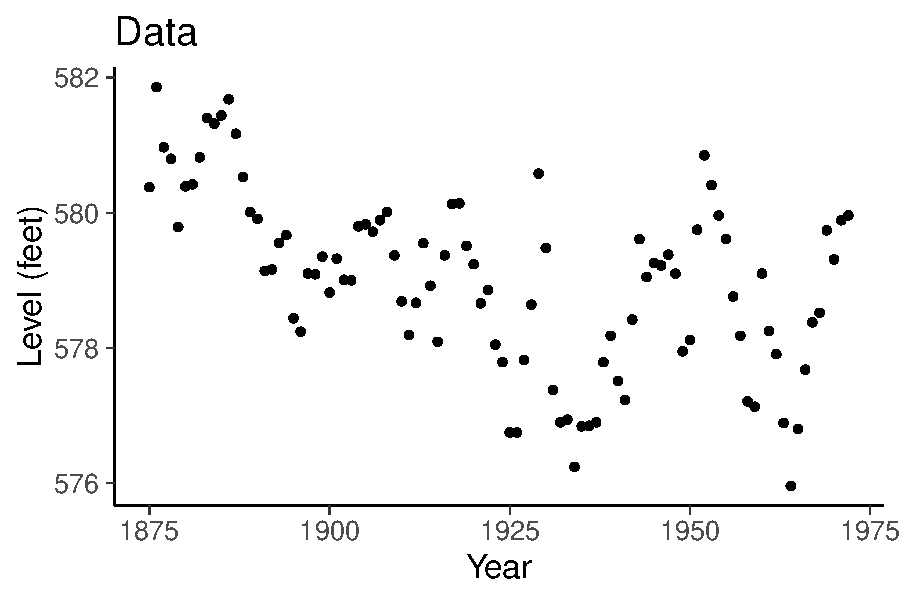
\includegraphics[width=10cm]{lake4data.pdf}}
  \only<2>{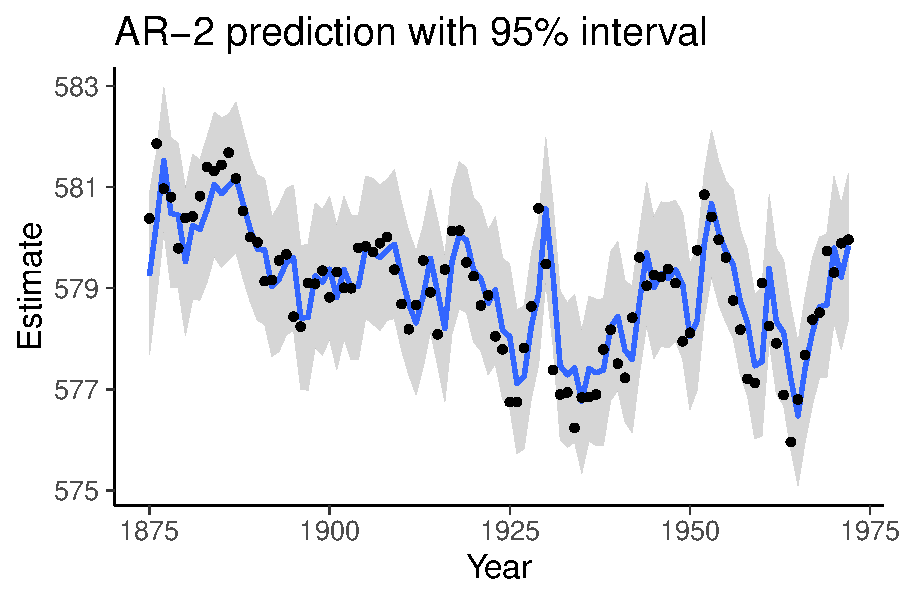
\includegraphics[width=10cm]{lake4pred.pdf}}
  \only<3>{\includegraphics[width=10cm]{lake4psisrefits.pdf}}

  \vspace{3\baselineskip}
  \only<3> {\small \url{mc-stan.org/loo/articles/loo2-lfo.html}}

  
\end{frame}

\begin{frame}{}
  
{\Large\color{navyblue} K-fold cross-validation}

\begin{list1}
\item K-fold cross-validation can approximate LOO
  \begin{list2}
    \item all uses for LOO
  \end{list2}
\item K-fold cross-validation can be used for hierarchical models
  \begin{list2}
    \item good for leave-one-group-out
  \end{list2}
\item K-fold cross-validation can be used for time series
  \begin{list2}
    \item with leave-block-out
  \end{list2}
\end{list1}

\end{frame}

\begin{frame}{}

  \only<1>{\includegraphics[width=10cm]{lake3kfoldbal1.pdf}}
  \only<2>{\includegraphics[width=10cm]{lake3kfoldbal2.pdf}}
  \only<3>{\includegraphics[width=10cm]{lake3kfoldrand.pdf}}
  \only<4>{\includegraphics[width=10cm]{rats1kfoldrand.pdf}}
  \only<5->{\includegraphics[width=10cm]{rats1oneratb.pdf}}
  \\
  \only<6>{kfold\_split\_random()\\ \vspace{0.2\baselineskip}
  kfold\_split\_balanced()\\ \vspace{0.2\baselineskip}
  kfold\_split\_stratified()}
  
\end{frame}

\begin{frame}{}

{\Large\color{navyblue} WAIC vs PSIS-LOO}

\begin{list1}
  \item<2-> WAIC has same assumptions as LOO
  \item<3-> PSIS-LOO is more accurate 
  \item<4-> PSIS-LOO has much better diagnostics
  \item<5-> LOO makes the prediction assumption more clear,\\ which
    helps if K-fold-CV is needed instead
  \item<6-> Multiplying by -2 doesn't give any benefit\\ (Watanabe
    didn't multiply by -2)
\end{list1}

\vspace{6\baselineskip}
{\small see \href{http://link.springer.com/article/10.1007/s11222-016-9696-4}{Vehtari, Gelman \& Gabry (2017a)}}
\end{frame}

\begin{frame}{}

{\Large\color{navyblue} *IC}

\begin{list1}
  \item AIC uses maximum likelihood estimate for prediction
  \item DIC uses posterior mean for prediction
  \item BIC is an approximation for marginal likelihood
  \item TIC, NIC, RIC, PIC, BPIC, QIC, AICc, ...
\end{list1}

\end{frame}

\begin{frame}{}

{\Large\color{navyblue} Marginal likelihood / Bayes factor}

\vspace{-0.3\baselineskip}
\begin{list1}
\item Like leave-future-out 1-step-ahead cross-validation but starting with 0 observations\\
  \onslide<3->{- which makes it very sensitive to prior}
  \onslide<4->{and \\- unstable in case of misspecified
    models}\uncover<5->{ also asymptotically}
\end{list1}
\vspace{-0.5\baselineskip}
  \onslide<2->{\includegraphics[width=9.4cm]{lake3bf.pdf}}

\end{frame}

\begin{frame}{}

{\Large\color{navyblue} Cross-validation for model assessment}

\begin{list1}
\item CV is good for model assessment when application specific utility/cost functions are used
  \begin{list2}
  \item e.g. 90\% absolute error
  \end{list2}
\item<2-> Also useful in model checking in similar way as posterior
  predictive checking (PPC)
  \begin{list2}
  \item model misspecification diagnostics\\ (e.g. Pareto-$k$ and p\_loo)
  \item checking calibration of leave-one-out predictive posteriors
    (ppc\_loo\_pit in bayesplot)
  \end{list2}
  {\small see demos \url{avehtari.github.io/modelselection/}}
\end{list1}

\end{frame}

\begin{frame}
  
   {\Large\color{navyblue} Radon example}

   PSIS-LOO diagnostics
   \includegraphics[width=.8\textwidth]{radon1k.pdf}

{\small see \href{http://link.springer.com/article/10.1007/s11222-016-9696-4}{Vehtari, Gelman \& Gabry (2017a)}}
   
 \end{frame}


\begin{frame}
  
{\Large\color{navyblue} Sometimes cross-validation is not needed}

\vspace{-0.5\baselineskip}

  \begin{list1}
  \item<2-> Posterior predictive checking is often sufficient\\
    \vspace{0.5\baselineskip}
    \includegraphics[width=11cm]{mesquite_ppc.pdf}\\
  \vspace{-0.1\baselineskip} {Predicting the yields of mesquite bushes.\\
    \color{gray} \footnotesize
    Gelman, Hill \& Vehtari (2020): Regression and Other Stories, Chapter 11.}\\
  \vspace{-0.8\baselineskip}
\end{list1}
{\footnotesize
  \begin{list2}
  \item<3-> BDA3, Chapter 6
  \vspace{-0.6\parskip}
  \item<3-> Gabry, Simpson, Vehtari, Betancourt, Gelman
    (2019). Visualization in Bayesian workflow. JRSS A, \url{https://doi.org/10.1111/rssa.12378}
  \vspace{-0.6\parskip}
  \item<3-> \url{mc-stan.org/bayesplot/articles/graphical-ppcs.html}
  \vspace{-0.6\parskip}
  \item<3-> \url{betanalpha.github.io/assets/case_studies/principled_bayesian_workflow.html}
   \end{list2}}
\end{frame}

% \begin{frame}{}

% {\Large\color{navyblue} Model comparison}

% \begin{list1}
% \item ``A popular hypothesis has it that primates with larger brains
%   produce more energetic milk, so that brains can grow quickly'' (from
%   Statistical Rethinking)
%   \begin{list2}
%     \item Model 1: formula = kcal.per.g $\sim$ neocortex
%     \item Model 2: formula = kcal.per.g $\sim$ neocortex + log(mass)
%   \end{list2}
% \end{list1}

% \vspace{10\baselineskip}
% {\small \url{mc-stan.org/loo/articles/loo2-example.html}}

% \end{frame}

% \begin{frame}

%   \only<1-2>{\includegraphics[width=10cm]{milkelpdloo.pdf}}
%   \only<3>{\includegraphics[width=10cm]{milkelpdloo2.pdf}}
%   \\
%   \only<2-3>{Model 1 elpd\_loo $\approx$ 3.7, SE=1.8\\
%   Model 2 elpd\_loo $\approx$ 8.4, SE=2.8}

% \end{frame}

% \begin{frame}[fragile]

%   {\includegraphics[width=10cm]{milkelpddiff.pdf}}
%   \\
%   {\scriptsize
% \begin{lstlisting}
% Model comparison: 
% (negative 'elpd_diff' favors 1st model, positive favors 2nd) 

% elpd_diff        se 
%       4.7       2.7 
% \end{lstlisting}}

% \end{frame}

% \begin{frame}

%   {\Large\color{navyblue} Arsenic well example -- Model comparison}

   
%    \includegraphics[width=.8\textwidth]{arsenic12d.pdf}

%    An estimated difference in ${\rm elpd}_{\rm loo}$ of 16.4 with SE of 4.4.
   
% {\small see \href{http://link.springer.com/article/10.1007/s11222-016-9696-4}{Vehtari, Gelman \& Gabry (2017a)}}
% \end{frame}

\begin{frame}{}

  {\Large\color{navyblue} Arsenic well example -- Model comparison}

\begin{list1}
\item Probability of switching well with high arsenic level in rural Bangladesh
  \begin{list2}
    \item Model 1 covariates: log(arsenic) and distance
    \item Model 2 covariates: log(arsenic), distance and education level
  \end{list2}
\end{list1}

\vspace{10\baselineskip}
{\small Gelman, Hill \& Vehtari (2020): Regression and Other Stories, Chapter 13.}

\end{frame}

\begin{frame}

  {\Large\color{navyblue} Arsenic well example -- Model comparison}
  
  {\includegraphics[width=6.5cm]{arsenicelpdloo.pdf}}
  % \only<3>{\includegraphics[width=10cm]{milkelpdloo2.pdf}}
  \\
  {Model 1 elpd\_loo $\approx$ -1952, SE=16\\
  Model 2 elpd\_loo $\approx$ -1938, SE=17}

\end{frame}

\begin{frame}[fragile]

  {\Large\color{navyblue} Arsenic well example -- Model comparison}

  {\includegraphics[width=6.5cm]{arsenicelpddiff.pdf}}
  \\
  {\scriptsize
\begin{lstlisting}
> loo_compare(model1, model2)
       elpd_diff se_diff
model2   0.0       0.0  
model1 -14.4       6.1  
\end{lstlisting}}
\vspace{-\baselineskip}
    {\scriptsize \hspace{6cm} see \href{http://link.springer.com/article/10.1007/s11222-016-9696-4}{Vehtari, Gelman \& Gabry (2017a)}}
    
\end{frame}

% \begin{frame}
  
% {\Large\color{navyblue} Sometimes cross-validation is not needed}

% \vspace{-0.5\baselineskip}

%   \begin{list1}
%   \item Posterior predictive checking is often sufficient\\
%     \vspace{0.5\baselineskip}
%     \includegraphics[width=11cm]{mesquite_ppc.pdf}\\
%   \vspace{-0.1\baselineskip} {Predicting the yields of mesquite bushes.\\
%     \color{gray} \footnotesize
%     Gelman, Hill \& Vehtari (2019): Regression and Other Stories, Chapter 11.}\\
%   \vspace{-0.8\baselineskip}
% \end{list1}
% {\footnotesize
%   \begin{list2}
%   \item BDA3, Chapter 6
%   \vspace{-0.6\parskip}
%   \item Gabry, Simpson, Vehtari, Betancourt, Gelman
%     (2019). Visualization in Bayesian workflow. JRSS A, \url{https://doi.org/10.1111/rssa.12378}
%   \vspace{-0.6\parskip}
%   \item \url{mc-stan.org/bayesplot/articles/graphical-ppcs.html}
%   \vspace{-0.6\parskip}
%   \item \url{betanalpha.github.io/assets/case_studies/principled_bayesian_workflow.html}
%    \end{list2}}
% \end{frame}

\begin{frame}[fragile]

  {\Large\color{navyblue} Arsenic well example -- Model comparison}

  {\scriptsize
\begin{lstlisting}
> loo_compare(model1, model2)
       elpd_diff se_diff
model2   0.0       0.0  
model1 -14.4       6.1  
\end{lstlisting}}

    {\tt se\_diff} and normal approximation for the uncertainty in the
    difference is good only if models are well specified and the
    number of observations is relatively big (more details in a
    forthcoming article).
    
%\vspace{9\baselineskip}
%    {\scriptsize \hspace{6cm} see \href{http://link.springer.com/article/10.1007/s11222-016-9696-4}{Vehtari, Gelman \& Gabry (2017a)}}
    
\end{frame}


\begin{frame}{}

{\Large\color{navyblue} Sometimes cross-validation is not needed}

\begin{list1}
\item<+-> For some very simple cases you may assume that true model
  is included in the list of models considered ($M$-closed)
  \begin{list2}
  \item<+-> see predictive model selection in $M$-closed case by
    San Martini and Spezzaferri (1984)
  \item<+-> but you should not force your design of experiment or
    analysis to stay in the simplified world
  \end{list2}
% \item<+-> For fully non-parametric models you may assume that true model
%   is included in the list of models considered ($M$-closed)
%   \begin{list2}
%   \item<+-> related to talk by Chris Holmes
%   \item<.-> see
%     \href{http://dx.doi.org/10.1214/12-SS102}{Vehtari \& Ojanen
%       (2012)} for earlier references
% \item<+-> posterior convergence rate can be slow for fully non-parametric models
% \end{list2}
\item<+-> In nested case, often easier and
  more accurate to analyse posterior distribution of more complex
  model directly \\
  {\small \url{avehtari.github.io/modelselection/betablockers.html}}
   % \begin{list2}
   %   \item<3-> need to do some model checking anyway
   % \end{list2}
\end{list1}

\end{frame}

\begin{frame}{}

  {\Large\color{navyblue} Sometimes predictive model comparison can be useful}

      \begin{minipage}[t]{0.45\linewidth}
        \begin{center}
          \includegraphics[width=5cm]{fitg2_xx_areas.pdf}\\
          Marginal posterior intervals
        \end{center} 
      \end{minipage}
      \pause
      \begin{minipage}[t]{0.45\linewidth}
        \begin{center}
          \includegraphics[width=5cm]{fitg2_xx_scatter.pdf}\\
          Joint posterior density
        \end{center} 
      \end{minipage}

            \begin{center}
      {\scriptsize rstanarm + bayesplot}
    \end{center}

    \pause
    {\small
      see also \href{https://avehtari.github.io/modelselection/collinear.html}{Collinear demo}
    }

\end{frame}

\begin{frame}{}

  {\Large\color{navyblue}  What if one is not clearly better than others?}

  \begin{list1}
  \item<2-> Continuous expansion including all models?
    \begin{list2}
    \item and then analyse the posterior distribution directly\\
        {\small \url{avehtari.github.io/modelselection/betablockers.html}}
      \item sparse priors like regularized horseshoe prior instead of variable selection\\
        {\small video, refs and demos at
          \url{avehtari.github.io/modelselection/}}
    \end{list2}
  \item<3-> Model averaging with BMA or Bayesian stacking?\\
    {\small \url{mc-stan.org/loo/articles/loo2-example.html}}
  \item<4-> In a nested case choose simpler if assuming some cost for
    extra parts?\\
    {\small \url{andrewgelman.com/2018/07/26/parsimonious-principle-vs-integration-uncertainties/}}
  \item<5-> In a nested case choose more complex if you want to take
    into account all the uncertainties.\\
    {\small \url{andrewgelman.com/2018/07/26/parsimonious-principle-vs-integration-uncertainties/}}
  \end{list1}

\end{frame}

\begin{frame}

  {\Large\color{navyblue} Model averaging}
  
  \begin{list1}
  \item<+-> Prefer continuous model expansion
  \item<+-> If needed integrate over the model space = model averaging
  \item<+-> Bayesian stacking may work better than BMA
    \begin{list2}
    \item \href{https://projecteuclid.org/euclid.ba/1516093227}{Yao, Vehtari, Simpson, \& Gelman (2018)}
    \end{list2}
  \end{list1}
  
\end{frame}

\begin{frame}{}

  {\Large\color{navyblue}  Cross-validation and model selection}

  \begin{list1}
  \item<1-> Cross-validation can be used for model selection if
    \begin{list2}
      \item small number of models
      \item the difference between models is clear
    \end{list2}
  \item<2-> Do not use cross-validation to choose from a large set of models
    \begin{list2}
    \item selection process leads to overfitting
    % \item you may use projection predictive approach
    % \item useful when correlating variables make the posterior
    %   distribution analysis difficult\\
    %   {\small video, refs and demos  at \url{avehtari.github.io/modelselection/}\\
    %   and \href{http://link.springer.com/article/10.1007/s11222-016-9649-y}{Piironen \& Vehtari (2017)}}
    \end{list2}
  \item<3-> Overfitting in selection process is not unique for cross-validation
  \end{list1}
\end{frame}

\begin{frame}
  
  {\Large\color{navyblue} Selection induced bias and overfitting}

  \begin{itemize}
  \item Selection induced bias in cross-validation
    \begin{itemize}
    \item same data is used to assess the performance and make the selection
    \item the selected model fits more to the data
    \item the CV estimate for the selected model is biased
    \item recognized already, e.g., by Stone (1974)
    \end{itemize}
    \pause
  \item Performance of the selection process itself can be assessed
    using two level cross-validation, but it does not help choosing
    better models
    \pause
  \item Bigger problem if there is a large number of models as in
    covariate selection
  \end{itemize}

\end{frame}

\begin{frame}

  {\Large\color{navyblue} Selection induced bias in variable selection}

  \includegraphics[width=\textwidth]{cv.pdf}

\end{frame}

\begin{frame}

  {\Large\color{navyblue} Selection induced bias in variable selection}

  \includegraphics[height=0.88\textheight]{simulated_searchpath.pdf}
   \vspace{-1.5\baselineskip}
   \mbox{{\hspace{8cm} \footnotesize \href{http://link.springer.com/article/10.1007/s11222-016-9649-y}{Piironen \& Vehtari (2017)}}}

\end{frame}

% \begin{frame}

%   {\Large\color{navyblue} Selection induced bias in variable selection}

%   \includegraphics[height=0.88\textheight]{simulated_variability.pdf}
%    \vspace{-1.5\baselineskip}
%    \mbox{{\hspace{8cm} \footnotesize \href{http://link.springer.com/article/10.1007/s11222-016-9649-y}{Piironen \& Vehtari (2017)}}}

% \end{frame}

% \begin{frame}

%   {\Large\color{navyblue} Selection induced bias in variable selection}

%   \includegraphics[height=0.88\textheight]{real_searchpath.pdf}
%    \vspace{-2\baselineskip}
%    \mbox{{\hspace{9.5cm} \parbox[t]{12cm}{\footnotesize \href{http://link.springer.com/article/10.1007/s11222-016-9649-y}{Piironen \&\\ Vehtari (2017)}}}}

% \end{frame}

\begin{frame}{}

  {\Large\color{navyblue}  Take-home messages}

  \begin{list1}
  \item It's good to think predictions of observables, because
    observables are the only ones we can observe
  \item \only<1>{\color{gray}}Cross-validation can simulate predicting and observing new
    data
  \item \only<2>{\color{gray}}Cross-validation is good if you don't
    trust your model
  \item \only<3>{\color{gray}}Different variants of cross-validation
    are useful in different scenarios
  \item \only<4>{\color{gray}}Cross-validation has high variance, and
    {\bf if} you trust your model you can beat cross-validation in
    accuracy
  \end{list1}
  \only<5>{~}

\end{frame}

\end{document}

%%% Local Variables: 
%%% mode: latex
%%% TeX-master: t
%%% End:
